% !TeX spellcheck = en_GB

\chapter{Introduction}

Portals are typically used to accelerate rendering speed when used in \gls{pvs} algorithms \cite{luebke:1995:portals}. This can be crucial for applications, which need to visualize scenes in real time, such as architectural walkthroughs, video games or \gls{vr} experience. It is a topic widely covered in literature.

However, a special kind of portals, the transformative portals, are less commonly seen. While regular portals are use to improve performance, transformative portals offer visualization and interaction possibilities. When present, they are typically very visible to the user. In video games, they can allow for interesting gameplay interaction, seamless transition between worlds \cite{schmalstieg:1999:sewing}. For \gls{vr} they off new possibilities for locomotion. Lastly, although they are not quite portals, magic lenses are very similar to transformative portals and allow for useful visualisations \cite{viega:1996:3d}.

\section{Portal definition}
Before further discussing portals a definition is needed: Our world can be seen as one big space that is divided into multiple subspaces by large objects. For instance walls which split up a house into multiple rooms. A portal connects two subspaces, similar to a door connecting two rooms. Through a portal the connected subspace can be seen. To reach the other subspace one must traverse through the portal.

\subsection{Transformative Portals}
Regular portals can only connect subspaces that are adjacent to each other. Travelling through a regular portal cannot be faster, than reaching a place by going in a straight line.

For transformative portals however, there are no such limitations. Transformative portals can connect completely arbitrary subspaces and may even connect a subspace to itself. In the presence of transformative portals a straight path may not be the shortest, as travelling through a portal could be faster. Transformative portals are similar to wormholes described by \textcite{Visser:Wormholes} in his book.

\subsection{Portal Recursion}
When looking through a portal parts of the connected subspace can be seen. In that subspace there could be another portal through which yet another subspace is visible. In this example  two recursions are needed to see the final subspace. In reality this could continue indefinitely. However, due to technical reasons, there is often a limit to the number of recursions. In this paper this limit is referred to as \gls{recursioncount}. A recursion count of 0 means that no other subspaces can be seen through portals. A recursion count of 1 allows looking through portals, but portals in connected subspaces can not be looked through.

\section{Research Question}

In this paper the rendering of transformative portals is investigated. A prototype implementation will be built testing various optimizations. The performance of this prototype will be measured to find bottlenecks, which can be addressed in future works. Furthermore, transformative portals are covered only sparingly in literature, especially in the context of video games. This thesis may not be fully exhaustive, but can provide a good starting point for future transformative portal implementers.


\chapter{Graphics programming}

Many algorithms describe in later sections use computer graphics techniques or special features of the graphics cards. This sections serves as a quick summary of some of these features and techniques, so the later parts of this thesis can be better understood. 


\section{Ray Tracing}
Ray tracing is a rendering technique, which creates an image by casting rays into the scene. These rays will be referred to as \glspl{viewray}. For each pixel a ray is cast and checked for intersections with objects in the scene. The colour of an intersected object at the corresponding intersection point decides the colour of the pixel cast by the ray \cite{bungartz:2002:einfuhrung}. This technique can also be extended. For example from the intersection point additional rays can be casted in the directions of all the lights. If the first intersection is not the light the object lies in a shadow \cite{whitted:2005:improved}. Raytracing can also be used to implement portals in an intuitive way. When a \gls{viewray} intersects with one \gls{endpoint} the view ray is recast from the other \gls{endpoint}.

Ray tracing is well known for being able to produce images with higher quality, compared to rasterization based rendering. But it is also known for being quite expensive and mostly used for offline rendering. However, \textcite{wald:2001:interactive} have shown that in some cases software ray tracing can  outperform rasterization approaches for lower resolutions with a high triangle count \cite{wald:2001:interactive}.

Ray tracing is not limited to the \gls{cpu}, there exist many ray tracing applications for the \gls{gpu} as well such as the works of \textcite{foley:2005:kd} or \textcite{parker:2010:optix}. With the introduction of Nvidia's RTX \glspl{gpu} ray tracing can now be supported in hardware \cite{raytracinggems}.


\section{GPU Features / Pipeline}

This section gives a quick overview over\gls{gpu} features used in the implementation. The implementation uses the Vulkan \gls{api} with version 1.1. Although many graphic \glspl{api} work similarly, the following sections only refer to Vulkan 1.1 unless otherwise noted.


\subsection{Vertex Processing}

The first step in the \gls{gpu} pipeline is vertex processing, via programmable vertex shaders. Vertices are transformed to their correct location using matrices. The vertex processing stage is also responsible for projecting a vertex's position into clip space via a projection matrix. Additional attributes, such as normals or texture coordinates can be set, which can be used in later stages. After vertex processing, individual vertices are assembled to primitives according to the primitive topology. These primitives may be further processed. This can be done with an optional geometry shader, tessellation control shader and tessellation evaluation shader \cite{akine:2018:realtime, khronos:vulkan:spec1.1}. However, the implementation will only use vertex shaders.


\subsection{Clipping}
\label{section:clipping}

Not every primitive is visible on the screen, only those which are at least partially inside the view volume. Primitives wholly inside the view volume are just passed to the rasterizer. Primitives outside will be discarded. For primitives partially inside the view volume clipping needs to be performed. The primitive is cut against the view volume, discarding outside vertices and creating new ones at the intersection with the view volume. The clipping is performed in clip space, before the perspective division using  four-dimensional homogenous position vectors. This allows the use of linear interpolation to calculate the new vertices' position, which would not be possible in perspective space. The view volume is often defined as the unit cube, ranging from (-1,-1,-1) to (1,1,1).
\cite{akine:2018:realtime}. However, this can be configured and differ for graphic \glspl{api}. For example, in Vulkan the view volume ranges from (-1,-1,0) to (1,1,1) by default \cite{khronos:glsl4.60:spec}.

The view volume is defined by 6 clip planes. A clip plane divides the space into an inside space and an outside space.
In addition to the 6 clip planes, which define the view volume, additional clip planes can be provided by the user \cite{akine:2018:realtime}. In Vulkan 1.1 and OpenGL 4.6 this can be achieved by setting values in the \textit{gl\_ClipDistance} array in a \gls{glsl} vertex or geometry shader. Each value defines the signed distance to the corresponding user-defined clip plane. A negative value indicates that the point is outside, while a positive value indicates that it is inside.  Primitives are clipped against all clip planes and only parts that are inside for all planes remain \cite{khronos:vulkan:spec1.1, khronos:openGL:spec4.6}.

\subsection{Screen Mapping}
After clipping and the perspective divide all primitives' coordinates are in \textit{normalized device coordinates} and inside the range defined by the view volume. Before they are passed to the rasterizer the \textit{normalized devices coordinates} are mapped to \textit{frame buffer coordinates}/\textit{screen coordinates}. This mapping is influenced by the viewport \cite{akine:2018:realtime, khronos:vulkan:spec1.1}.

For example in Vulkan the \textit{normalized device coordinates} range form (-1,-1,0) to (1,1,1). The x and y coordinates are multiplied by half of the viewports width and height respectively. Then the view port's center is added. The z coordinate is multiplied by maximum depth minus minimum depth, then the minimum depth gets added to the result. \cite{khronos:vulkan:spec1.1}.

\subsection{Polygon Rasterization}
Although it is possible to rasterize points and lines, this section will only cover polygon rasterization, as only polygon rasterization will be used in the implementation.

First the winding order of the polygon is determined. Then depending on the front face settings, clock wise or counter clock wise, the polygon is either front or back facing. All polygons that are not front facing count as back facing, including zero-area polygons. Depending on the active cull mode, the polygon may be culled depending on the way it is facing. The cull mode can be no culling, cull front faces, cull back faces or cull all faces \cite{akine:2018:realtime, khronos:vulkan:spec1.1}.

If the polygon is not culled, fragments will be created for pixels, with a sample point inside the polygon. If the sample point lies on a polygon edge the following rule applies: For two polygons and a sample point on their common edge, exactly one fragment is created. The fragments attributes are then calculated, using a convex combination of the polygon's vertices. Fragments with a sample location at a vertex location will have exactly that vertex's attributes. Other fragments' attributes are calculated via a linear combination of attributes of the polygon's vertices. The linear combination's scalars depend on the sample position within the polygon \cite{akine:2018:realtime, khronos:vulkan:spec1.1}.

Instead of a linear combination a attribute can be annotated  as \textit{flat}. In this case the value of the polygon's \textit{provoking vertex} is used directly an no interpolation is performed. The provoking vertex is generally the first vertex of a primitive and depends on the primitive topology \cite{akine:2018:realtime, khronos:vulkan:spec1.1}.

\subsection{Early Per Fragment Tests}
Before fragments are passed to the fragment processing stage, various test are performed, which may discard the fragment. One such a test would be the scissor test, which tests if a given fragment is inside a specified rectangle. If it is outside the fragment is discarded. Some tests can happen early or late, depending on the fragment shader. Examples would be the depth and stencil test, which are explained in later sections \cite{khronos:vulkan:spec1.1}.

\subsection{Fragment Processing}
Every fragment the passes all the early fragment tests is passes to the fragment shader. Usually the fragment shader uses a fragments attributes to decide which colour to output.
It can also use other data, which is not specific to a fragment, such as storage buffers (see section \ref{section:buffer}). However, it does not need to output anything or actual colour values. Furthermore the fragment shader can also perform writes to storage buffers in addition or instead of outputting a colour. For a pixel location multiple fragments can be created. A fragment shader's colour output does not neccessarily influence the final image. The output can be overridden by later fragments at the same pixel location or discarded by late tests.


\subsection{Depth Test}
\label{section:depthtest}
Without the \gls{gpu}['s] depth test objects would need to be drawn according to the painter's algorithm: First they are sorted by their distance to the camera. Then they are drawn back to front writing their colour to the corresponding pixels. The object farthest away is drawn first and the nearest object is drawn last. Otherwise objects that are behind other objects may be drawn over them, leading to wrong images. However, there are cases where the painter's algorithm does not work, for example when three objects overlap each other \cite{akine:2018:realtime}.

The depth test offers a solution to this problem, as well as removing the need for the painter's algorithm. Before the colour output of a fragment is written to a pixel the depth test is performed. The current fragment's depth value is compared to the depth value of the fragment, which was last written to that location.
%The depth value of the last written fragment is stored inside the depth buffer.
If the current fragment depth value is not farther from the view point than the last fragment, the current fragment is discarded. Otherwise it writes its values as usual and stores its depth in the depth buffer. The write to the depth buffer is part of the test, but may be disabled. The depth buffer is sometimes also called z-buffer \cite{akine:2018:realtime}.

For Vulkan the depth values range from 0 to 1. In many applications lower values are used to indicated near values. But it does not need to be that way. In contrary, using high depth values for near objects is better in some cases, but never worse. For perspective view, the depth values however are not linearly distributed. The difference in depth value between two objects becomes smaller, the further both are away from the view. At some point the difference becomes so smaller than expressible using floating point values. They will have the same depth value, even though they are differently far away. This results in visual flickering as those objects randomly occlude each other. This is called z-fighting. However, when values close to 0 are used for far away objects, these objects can be make use of the increased precision of floating point values near 0. This increased precision helps to mitigate z-fighting. It is also possible that normalized values are used to store depth, which have a constant precision within their range. In this case using an inverse z-buffer will not perform any worse than the alternative \cite{lapidous:1999:optimal, nvidia:inversez}.

The depth test comparison operation can be configured and should correspond to the depth buffer usage. A inverse depth buffer would use the opposite comparison of what a regular depth buffer would use. The following comparisons are possible \cite{sellers:vulkanprogramming}:
\begin{itemize}
	\item The test always passes
	\item The test never passes
	\item Pass if new depth is less than the old value
	\item Pass if new depth is less than or equal to  the old value
	\item Pass if new depth is equal to the old value
	\item Pass if new depth is not equal to the old value
	\item Pass if new depth is greater than the old value
	\item Pass if new depth is greater than or equal to  the old value	
\end{itemize}

The write to the depth buffer is part of the test, but it be configured to not write the new value. Additionally the new depth value may be influenced before the test, with a depth bias \cite{sellers:vulkanprogramming}.

\subsection{Stencil Test}
\label{section:stenciltest}

The stencil test serves as another way to discard a fragment. It uses a stencil buffer to store stencil values, similar to the depth buffer. In fact both buffers are stored alongside each other in one attachment and cannot be separated. This is called the depth stencil attachment. The stencil test compares a reference value, with the value inside the stencil buffer at the fragments location. If the test fails, the fragment is discarded. Different reference values and comparison operations can be configured. The same comparisons from the depth test can be used. Additionally the stencil test can change the contents of the stencil buffer. The following operations are possible \cite{sellers:vulkanprogramming}:
\begin{itemize}
	\item Keep the value of the stencil buffer
	\item Set the value to 0
	\item Replace the the stencil value with the reference value
	\item Increment the stencil value and clamp it at the maximum value
	\item Decrement the stencil value and clamp it at 0
	\item Invert the bits of the stencil value
	\item Increment the stencil value and wrap around
	\item Decrement the stencil value and wrap around	
\end{itemize}

It is possible to use a different operation depending on the outcome of the depth and stencil test. A different operation can be configured for: stencil failed, stencil passed but depth failed, both tests passed. The test and operations can be different for back and front faces \cite{sellers:vulkanprogramming}. Additionally, a compare and a write mask can be configured. Before the test the reference value and the stencil buffer value are bitwise AND-ed. The write mask selects the bits of the stencil values that are updated. In Vulkan 1.1 the stencil buffer can only have exactly 8 bits or not be present at all. There is no texture format available for depth stencil attachment that allows a different number of bits \cite{khronos:vulkan:spec1.1}.

\subsection{Early Depth Stencil Test}
Although the depth and stencil test are defined to run after the fragment shader, they can actually happen before the fragment shader is executed. When possible this happens automatically. This improves performance as early discarded fragments do not need to invoke or be processed by the fragment shader. However, this is not always possible In the following cases the test happens late \cite{sellers:vulkanprogramming}:

Firstly, when the fragment shader can update the depth value, the actual depth value cannot be known before executing the shader. Secondly, when the shader has side effects, such as writing into a storage buffer. Discarding early would prevent the write from happening. Lastly, when the shader could discard the fragment, as discarding should prevent updating the depth buffer \cite{sellers:vulkanprogramming}.

 It is possible to force the fragment test to run early. In \gls{glsl} this is done via the following line in the fragment shader \cite{khronos:glsl4.60:spec}:
\begin{lstlisting}
layout(early_fragment_tests) in;
\end{lstlisting}


\subsection{Instanced Drawing}
In some cases applications may be limited by the amount of commands they can send to the \gls{gpu}. One way to reduce the amount of commands is to used instanced drawing. When using instanced drawing the same model can be drawn multiple times. Each of those models may receive different per instance data. Additionally shaders can query the instance id to perform different logic for each instance \cite{akine:2018:realtime}. One example is for drawing gras. Instead of issuing a draw for each blade of gras, just one instanced draw can be issued. Each instance is then draw at a different location using different matrices for each instance.


\subsection{Occlusion Queries}
A occlusion query is a way to count the number of fragments that pass all fragment tests. The query counts all fragments for all rendering commands between the start and the end of the occlusion query. The performance of the query can be improved by configuring it to be less precise \cite{akine:2018:realtime}. For example in Vulkan a occlusion query by default returns 0 if no fragment was drawn and a arbitrary non zero value if at least one fragment is drawn. This specification allows Vulkan to use the more efficient query when available and otherwise fall back to the exact query. To enable precise precision queries the flag \textit{VK\_QUERY\_CONTROL\_PRECISE\_BIT} must be passed to the function that starts the query \cite{khronos:vulkan:spec1.1}.

Occlusion queries have many applications. One important use case is for occlusion culling. Complex geometry is approximated by a simple bounding volume, which is much less expensive to draw. First a part of a scene is drawn, but only to the depth buffer. Then the bounding volume is drawn with an active occlusion query. If no fragment passed the test, the bounding volume is either occluded or not in the view volume. The same is true for the complex geometry, which can then be skipped in such a case. Occlusion queries have a very high latency, so the time saved by occlusion culling must be worthwhile \cite{akine:2018:realtime, sellers:vulkanprogramming}.

\section{OpenGL and GLSL}
OpenGL is short for Open Graphics Library and is a cross platform \gls{api} for graphics hardware. It is and open standard of the Khronos Group. OpenGL defines a set of commands available to a programmer. This set of commands are implemented by driver implementers for specific \gls{gpu}. This way programmer does not need to know which \gls{gpu} will be used in the program and only need to program against the OpenGL \gls{api}. Some operations on the \gls{gpu} are fixed and can only have their settings configured. Other operations are fully programmable using shaders, which are small programs executed on the \gls{gpu} \cite{khronos:glsl4.60:spec}.

\Gls{glsl} is a human readable programming language for defining OpenGL shaders and is very similar to the C programming language. \Gls{glsl} is a actually set of very close languages, for each programmable part of the graphics pipeline. Some keywords are only available in a subset of those languages. There is a small amount of built in variables that influence the pipeline or are made available for use in the shader \cite{khronos:glsl4.60:spec}.


\section{Vulkan}
Vulkan is very similar to OpenGL and is also specified by the Khronos Group. It is designed for more explicit control of low-level graphics and compute functionality \cite{khronos:vulkan:spec1.1}. The implementation presented in this thesis uses Vulkan as its graphics \gls{api}. The following sections give a quick overview of important aspects of Vulkan.

\subsection{SPIR-V}

Shader code in Vulkan must be defined in \gls{spir} format \cite{khronos:vulkan:spec1.1}. \Gls{spir} is an intermediate language for shaders. It can also be used for compute kernels.  Shaders written in any shader language can be compiled to \gls{spir}, as long as corresponding compiler exists \cite{kessenich:2018:spir}. This implementation will use \gls{glsl} and compile it to SPIR-V. However, the \gls{glsl} for used for Vulkan is an extension to \gls{glsl}. Additional features are available and some are removed \cite{khronos:vulkan:glsl}. However, \gls{spir} is not limited to Vulkan. For example, it can be used for OpenGL instead of \gls{glsl} \cite{khronos:glsl4.60:spec}.

\subsection{Debugging with Validation Layers}

In Vulkan it is possible to intercept \gls{api} calls with the help of layers. The lowest layer is the core Vulkan \gls{api} defined by the specification. A higher layer can intercept all or a subset of calls for a lower layer. A higher layer can, but does not need pass on a call to its next lower layer. The core Vulkan layer assumes correct \gls{api} usage, resulting in undefined behaviour for incorrect usages for most cases. If error checking is needed it can be performed in validation layers. The Vulkan specification recommends developing applications with validation layers enabled to catch and eliminate errors. For shipping builds the validation layers should be disabled for improved performance \cite{khronos:vulkan:spec1.1}.


However, a validation layer is often not enough for debugging. Vulkan offers the debug utilities extension. One functionality of this extension is to annotated vulkan objects, such as textures, with user defined names to help identifying them while debugging. Additionally, debug  messengers can be created to provided callbacks for the validation layers.
\cite{khronos:vulkan:spec1.1}

\subsection{Device Memory}
Many resources in Vulkan, such as buffers and images, do not allocated memory. Instead device memory must be manually allocated and then bound to the specific resource. \Glspl{gpu} have different memory types of different size and properties. Some memory type may be fast to access by the \gls{gpu} or can be directly written by the \gls{cpu}. Some type can do both, but only has a very limited amount of memory. Furthermore, specific resources require specific properties. The memory types an their properties must be queried by the developer and can differ for each \gls{gpu}. The amount of allocations is limited so it is generally better to allocated huge chunks and bind different ranges to resources \cite{khronos:vulkan:spec1.1}.

\subsection{Image}
In contrast to buffers with a linear array data images have multi dimensional array of data. They can have up to 3 dimensions and can be used for various purposes, such as attachments or as texture. Instead of raw bytes images have individual elements defined by the image format. Image have a layouts which is initially specified and can transitioned be to other layouts. Each layout has different supported operations.
For example one layout allows the image to be used as colour attachment serving as a fragment shader output. The exact memory layout is not known and is implementation defined and depends on the image layout. 
Images cannot be directly accessed by shaders. Instead image views are used, which specify contiguous ranges with an image and contain additional metadata.   \cite{khronos:vulkan:spec1.1}.

\subsection{Buffer}
\label{section:buffer}
A buffer is a resource that can be created and represents unformatted linear array of bytes. They can be used for various purposes, by providing data to the shader or to certain commands. When creating a buffer its intended usage must be specified. One use case of a buffer is in form of a \gls{ubo} or storage buffer descriptor. \Glspl{ubo} can be used to provide shaders with read only data size, while a storage buffer provides read and write access \cite{khronos:vulkan:spec1.1}.

\subsection{Renderpass}
\label{section:renderpass}

%TODO Explain: Attachments

The renderpass represents attachments, subpasses and their dependencies. For each attachment a renderpass needs an \textit{attachment description}. This description contains the attachment's format, sample count and how its contents are treated at the beginning and end of the renderpass \cite{khronos:vulkan:spec1.1}.

A subpass describes  one part of the renderpass. A renderpass may one or more subpass. It describes how the attachments are used in the subpass. A subpass can use attachments as input, as output, preserve them as well as performing resolve operation on them, for multi sampling applications. A subpass can have multiple input, output, preserve and resolve attachments, but only one depth stencil attachment. All subpasses render to the same dimensions. Fragments that write to an output attachment at a specific pixel coordinate may read from input attachments only at that coordinate \cite{khronos:vulkan:spec1.1}.

A subpass dependency describes which operations of a subpass depend on which operations of another subpass, in form of a execution and memory barrier. The actual execution of the subpasses may be reordered or overlap as long as it is allowed by the subpass dependencies. If an explicit pipeline barrier (see section \ref{section:synchronisation}) is used during a subpass, that subpass needs a dependency on itself \cite{khronos:vulkan:spec1.1}.

\subsection{Frame buffer}
The renderpass only defines how attachments are used, but does not define their dimensions or which concrete attachments are actually used. The image views which are used as attachments are defined by the frame buffer. They are specified when creating the frame buffer as well as the dimensions. A frame buffer is created, based on a specific renderpass. The frame buffer attachments match the requirements of that renderpass. The frame buffer can only be used with that specific renderpass or a compatible one \cite{khronos:vulkan:spec1.1}.


\subsection{Graphics pipeline}
A graphics pipeline defines the various settings for rendering an object. The shader stages define which shader modules to use, their type and their entry point. The vertex input state defines the vertex attributes as well as whether and how they are interleaved. The input assembly defines how the primitives are created from the vertices. This could be a triangle list, a triangle strip, a point list, etc. The viewport state defines the different viewports, their position, their resolution, min and max depth, as wells as the scissor rectangles used for the individual scissor tests \cite{khronos:vulkan:spec1.1}.

The rasterizer state defines a multitude of settings for rasterization, including fully disabling it: The polygon mode decides how a primitive is rasterized. It can be fully filled, only have its lines drawn for wireframe views, or just have its points drawn. The front face is set to clock-wise or counter-clock-wise to decide which vertex order represents the front facing primitives. The cull mode can be configured to cull nothing, front faces, back faces or both. This can improve performance, as the back faces of watertight meshes are always occluded by the mesh's front faces. Furthermore the depth values can be modified via depth bias and the line width can be set \cite{khronos:vulkan:spec1.1}.

The depth stencil state configures the stencil and depth test as described in section \ref{section:depthtest} and section \ref{section:stenciltest}. The colour blend state configures how and if the outputs are blended together as well as which colour channels can be written to. Regular blending may be performed or logical operations can be used \cite{khronos:vulkan:spec1.1}.

The tessellation state configures the number of control points a patch has, if tessellation is enabled. It is ignored if not shaders for tessellation control and tessellation evaluation are present. The multi sample state configures various multi sampling settings. Tessellation and multi sampling are not used in the implemented prototype \cite{khronos:vulkan:spec1.1}.

The graphics pipeline also references a pipeline layout. It describes the values, buffers and textures passed to the shader and how they should be accessed. A graphics pipeline also references a specific subpass within a renderpass\cite{khronos:vulkan:spec1.1}.

Whenever different settings are needed for drawing objects, an additional pipeline needs to be created. For example, if there are two objects which need different shaders, each of the objects needs its own pipeline to draw it. However, there are a few values that can be configured to be dynamically adjustable using dynamic state. Static settings for specified dynamic state are ignored during pipeline creation and must be set dynamically before rendering \cite{khronos:vulkan:spec1.1}.

\subsection{Queues and Command Buffers}
In Vulkan most commands are not sent directly to the \gls{gpu}. Instead the commands are recorded in a command buffer. Then this command buffer can be submitted to a queue for execution on the \gls{gpu}. Not all queues support all commands. Which commands a queue supports depends on its queue family index and the capabilities associated with this index. The most common queue capabilities are graphics, compute and transfer operations \cite{khronos:vulkan:spec1.1}.

%Command buffers can not be created directly. First a command pool must be created. During the construction of the command pool, the queue family index must be passed. Command buffers created from a command pool can only be used to submit to queues, which match their command pool


\subsection{GPU Synchronisation}
\label{section:synchronisation}
In Vulkan the order of command executions has only a few implicit guarantees. Without explicit dependencies commands may be executed in arbitrary order or even overlap. For this Vulkan provides the developer with a few different synchronisation mechanisms \cite{khronos:vulkan:spec1.1}.

%A fence can be used to wait on the \gls{cpu} until certain tasks have been executed on the \gls{gpu} and their results are visible.
A Fence enables the \gls{cpu} to wait until \gls{gpu} commands have executed and their results are visible. Fences can be in two states, signalled and unsignalled. Fences can be unsignalled from the \gls{cpu}. They can be passes as parameters to a queue submission command. After all commands of a submission have been executed and their results are visible the fence gets signalled. The \gls{cpu} can either query the state of the fence or wait until it gets signalled \cite{khronos:vulkan:spec1.1}.

A semaphore can be used to synchronize different batches of recorded commands  which are submitted to queues. Just as fences, they have two states: signalled and unsignalled. A semaphore can become signalled after the execution of a batch. The execution of a batch can wait until a semaphore gets signalled. With a semaphore it is possible to synchronize commands between two different queues, which is can not be done using other types of synchronisation \cite{khronos:vulkan:spec1.1}.

An event can be used for dependencies of commands submitted to the same queue or between the \gls{cpu} and queue. It cannot be used to synchronize two different queues. An event has two states: signalled and unsignalled. Events can be signalled and unsignalled on the \gls{cpu} as well as the \gls{gpu}. The \gls{gpu} can wait until a event becomes signalled. The \gls{cpu} cannot wait on a event, but it can query its current state \cite{khronos:vulkan:spec1.1}.

A pipeline barrier is a explicit command that defines a memory dependency between commands submitted to one queue or commands within the same subpass of a renderpass. The pipeline barrier's memory dependency can be very precisely configured. For example it can define a dependency between the write of a specific image and a read from it. Furthermore, pipeline barriers are used to perform an image layout transition and to transfer queue ownership of buffers and images \cite{khronos:vulkan:spec1.1}.

The last synchronisation mechanisms are render passes and subpasses, which are described in section \ref{section:renderpass} \cite{khronos:vulkan:spec1.1}.



\subsection{Push Constant}

Instead of using buffers to pass data to a shader, a push constant can be used instead. They do not require a buffer. Individual parts of push constants are be directly updated by recording \textit{pushconstants} into a command buffer. At the beginning of recording the command buffer the push constant's content is undefined. A push constant allows only for a small amount of data. Vulkan only requires a limit of 128 bytes, which is equivalent to the bytes needed for two 4x4 float matrices. However, push constant are expected to outperform memory-backed resource updates, which is useful for data that changes rapidly. One example would be model matrices which change for each drawn object. 


\chapter{Related Work}
This section covers works related to this thesis. First other works, which make use of portals are discussed. Then works with relate to, but do not use, portals are presented. Lastly, \gls{vfc} is covered, which is often seen used together with \gls{pvs} algorithms. Furthermore, a modified version of \gls{vfc} could provide future optimization possibilities for the implementation presented in this thesis.


\section{Potentially Visible Set}

One use case for portals is the calculation of \gls{pvs}. A \gls{pvs} can be used to determine which geometry could be visible. This can either be defined for a specific point or for a whole region or subspace. While it is more difficult to calculate the \gls{pvs} for a region, this information can be used for many locations. The information contained in \glspl{pvs} is very useful for occlusion culling. Only object which contribute to the final image need to drawn. Skipping invisible objects reduces the \gls{gpu}['s] workload, leading to better performance \cite{cohen:2003:survey}.

In \gls{pvs} algorithms the regions or subspaces are called \textit{cells}, which are connected by portals. A \gls{pvs} for a \textit{cell} describes which geometry is visible for that \textit{cell}. For a \textit{cell} all geometry within itself and within adjacent \textit{cell} it is connected to is potentially visible. However, it is also possible to see geometry in \textit{cells} which are not directly connected to the original \textit{cell} . Note that a \gls{pvs} is not required to be exact and can be overestimated \cite{cohen:2003:survey}.

To calculate point based \glspl{pvs}, \textcite{luebke:1995:portals} proposed an on-the-fly algorithm. It is  a variation of \textcite{jones:1971:new}'s work. A portal's vertices are projected into screen space. Then a axial 2D bounding box of those vertices is created. This box forms a conservative bound for the portal and is called  \textit{cullbox}. Whenever all screen space projected vertices of an object lie outside this \textit{cullbox} the object can safely be culled.  To improve performance an even more conservative estimate can be used Instead of each vertex only an objects bounding box could be projected.  For portal recursions the \textit{cullbox} is the intersection of all the portals' \textit{cullboxes} which are involved in the recursion \cite{luebke:1995:portals}. 


%\cite{yang:2014:walkthrough}

\section{Connecting virtual worlds}

\textcite{schmalstieg:1999:sewing} used portals, to connect different virtual worlds together. In their paper the portals were referred to as SEAMs. Previously teleportation was used to to travel between virtual worlds, which can be very disorienting. With their implementation the user could see where they will go to and transitions smoothly between worlds.


Their implementation drew the SEAMs in depth first order. The primary world is rendered object after object. When a SEAM is encountered, for each SEAM pixel  the stencil value is increased, the colour set to the clear colour and  depth value is set to infinitely far away. The stencil buffer is initially at 0. Then the secondary the whole secondary world or recursion 1 is rendered, but only where the stencil value is equal to 1. After the secondary world is rendered, the seam that triggered it is sealed. This was done by drawing the SEAM, but it only sets the depth to its depth and decreases the stencil buffer. When a SEAM is encountered in the secondary world, it uses the same process, but with the stencil reference for comparision being incremented by 1. This process continues until a limit is reached. The rendering of a world is only finished, when all its SEAMs and their worlds have been drawn and the SEAMs were sealed again. To reduce the amount of worlds that potentially need to be drawn,  an adapted version of \textcite{luebke:1995:portals} on the fly \gls{pvs} algorithm was used. SEAMs were treated as portals and virtual worlds as regions in the algorithm \cite{schmalstieg:1999:sewing}.

\section{Portal Textures}
In architectural walkthroughs geometry can be very complex. However, such scenes are typically split into multiple rooms or cells, and connected by doors or portals. This allows the use of portal based acceleration techniques \cite{aliaga:1997:architectural}.

Instead of using portal culling to selectively rendering the geometry, \textcite{aliaga:1997:architectural} propose an alternative approach. Only the current cell needs to be rendered and portals can be replaced by textures. The cost of drawing a texture is significantly lower than drawing the actual geometry. The portal textures can be pre computed or computed on demand \cite{aliaga:1997:architectural}. 

There is a balance between visual fidelity and performance that must be considered. If the texture is recreated every frame the technique would be almost pointless. If the textures are not created often enough the portal could look like a painting with no depth. Using pre computed images takes a considerable amount of memory. Furthermore, the transition between the portal texture and the actual geometry must be smooth, to avoid visual popping. \textcite{aliaga:1997:architectural} accomplish this by smoothly warping the geometry represented by the portal texture from its current incorrectly projected position to its correct one.

Instead of using one texture for a portal, multiple textures can be used. A texture often has not the same viewpoint a needed for the portal. This can be corrected by image warping techniques. A second texture may contain information not present in the first, and helps to improve visual quality. By using multiple texture the total amount of pre computed images can be reduced drastically, improving the viability of pre computing \cite{rafferty:1998:3d}.

\section{Transformative Portals in Games}
One area where portals, especially transformative ones, are interesting is in video games. However, many games do not render portals in a special way. Other subspaces cannot be seen through the portal and when entering the users are often brought to a loading screen. 

However, there are also games that render portals in ways similar to as in the implementation describe in this thesis. While many more games with transformative portals exist, this section will only cover the following games:
\begin{itemize}
	\item Portal and Portal 2
	\item Splitgate: Arena Warfare
	\item Antichamber
	\item Budget Cuts
	\item Manifold Garden
	
	
\end{itemize}

\subsection{Portal and Portal 2}
\textit{Portal} and \textit{Portal 2}, from there on referred as \textit{Portal}, gives the player control of a portal gun. With this gun players may place one orange and one blue portal on a wall. When both portals are placed, they are active and the player can see and traverse between them. In \textit{Portal} only two portals per player can exist. In \textit{Portal} the portals are used for solving puzzles. \textit{Portal} uses an recursion count of 2. However, infinite recursions are visible. Parts of the previous rendered frame are used, as the texture for the final portal to achieve this effect \cite{lecture:portalProblems}.

\subsection{Splitgate: Arena Warfare}
\textit{Splitgate: Arena Warfare}, from there on referred as just \textit{Splitgate}, uses a similar mechanic to \textit{Portal}. However, \textit{Splitgate} is a shooter game and the portals are used to outmanoeuvre opponents, instead of puzzle solving. Portals can only be placed on special walls. Portals must be very near and facing each other for recursion to be visible. In \textit{Splitgate} this can be avoided carefully placing these special walls. Furthermore only players can only look through their own portal. Enemy portals cannot be seen through \cite{splitgate}.

\subsection{Antichamber}
\textit{Antichamber} is another puzzle game. Although portals are not its main focus, it is noteworthy as they behave very differently. \textit{Antichamber}'s portals are called \textit{transporter windows}. Instead of moving through them, player teleport when the \textit{transporter window} fills their entire screen. However, the player will not notice the teleportation immediately, as their view is filled with the \textit{transporter window}. Only after turning or moving away the teleportation can be noticed \cite{antichamber}.

\subsection{Budgetcuts}
\textit{Budgetcuts} is a \gls{vr} stealth game. One important aspect of \gls{vr} games is their locomotion system. Moving with a joystick feels unnatural and can introduce motion sickness. In \textit{Budgetcuts} the player moves around the world with a translocator, but it works differently compared to the previous games. First the player can create a portal at another place using their translocator device. That place can be seen by looking through another portal, which is located at the translocator. If the player decides to move to the other portal, they can press a button. Then the portal at the translocator wraps around the player. When finished the player stands at the new location. Portals in \textit{Budgetcuts} are visible only and cannot be physically interacted with \cite{budgetcuts, gdc:budgetcuts}.

\subsection{Manifold Garden}
Lastly there is \textit{Manifold Garden}, which is, as the time of this writing, an unreleased game. The game has no actual portals, but the edge of the world acts as one. When moving to the edge of the world, the player gets teleported to the other edge. There is no visible seam at the edge. It looks as if the world continues and repeats itself. Willian Chyr, \textit{Manifold Garden}'s author, calls this effect \textit{3D World Wrapping}.




\section{Magic Lens}
Another topic that uses techniques similar to portal rendering are magic lenses. A magic lense is a region, which has a special operation applied. For instance these operation could be magnification, rendering in wireframe, changing colour \cite{bier:1993:toolglass}, changing time \cite{ryall:2005:temporal, tiesel:2009:composable} etc. . Magic lenses are a powerful tool for visualization  \cite{bier:1993:toolglass, tominski:2014:survey}.

While early works used 2D magic lenses \cite{bier:1993:toolglass} they are not restricted to 2D. \textcite{viega:1996:3d} extended the concept fo magic lenses to 3D. They  rendered objects multiple times with a different clip plane active. This way only specific parts of an object would be rendered and different operation could be active while rendering.

\textcite{ropinski:2004:real} extended the 3D magic lenses for arbitrary shapes. To selectively render parts, they used two depth buffers, similar to depth peeling techniques \cite{everitt:2001:interactive}.

\section{World in miniature}
\Gls{wim} is a user interface technique for \gls{vr}. In addition to the regular \gls{vr} view of the virtual world, the user additionally holds a miniature version of the world, the \gls{wim}, in their hands. The objects in the \gls{wim} are in sync with the real world. Objects moved in the real world move in the  \gls{wim} and vice versa \cite{stoakley:1995:virtual}. 

This allows the user to orient themselves, similar to a map. Furthermore, objects can easily manipulated with the \gls{wim}. This would otherwise be very difficult, as the world in \gls{vr} is typically in 1:1 scale. Most objects would be out of reach for the user \cite{stoakley:1995:virtual}.

In addition to moving objects with  the \gls{wim} objects it is also possible for user to move their own avatar. This allows them to move around in the virtual world. However, immediately updating the \gls{vr} view while moving the avatar is very disorienting. Users where found to be very focused on the \gls{wim} while manipulating it and any animation of the full scale world requires them to shift focus. A alternative solution is to let the user fly inside their avatar in the \gls{wim}, steadily scaling it and fading out the original full scale world. The old \gls{wim} becomes the new full scale world and a new \gls{wim} is created \cite{pausch:1995:navigation}.




\section{View Frustum Culling}
As described in section \ref{section:clipping} only a small part of scene needs to be rendered. Although clipping discards invisible primitive, before sending them to the rasterizer, it still had to process them. \Gls{vfc} is an acceleration algorithm, which finds invisible geometry and omits them from rendering \cite{assarsson:2000:optimized, akine:2018:realtime}.

This is often done via bounding volume hierarchies. Each object is a node in a tree with a bounding volume. Multiple (close) nodes are grouped in a composite node. It children are the grouped nodes and its bounding volume contain all bounding volumes of its child nodes. Nodes can again as another composite node and so forth. The last node whit has no parent forms the root of the bounding box hierarchy tree \cite{clark:1976:hierarchical, assarsson:2000:optimized, akine:2018:realtime}.

\Gls{vfc} starts with the root node. A nodes bounding volume is tested against the frustum. If it is outside, all of its children will also be outside. The node and its children will not processed further. If the node's bounding volume is fully inside all its children will be inside and no further testing is needed for the children. If the node's bounding volume intersects the the view volume, the test must continue for each child \cite{akine:2018:realtime}.

There are multiple algorithms for performing the test itself. \textcite{assarsson:2000:optimized} implemented a fast \gls{vfc} algorithm for hierarchies of \glspl{aabb} and \glspl{obb}, which tests against the world space frustum. The boxes are tested against each of the frustum's clip planes, resulting in either inside, outside or intersecting. If the \gls{aabb} is outside of one plane, the test immediately stops and reports \textit{outside} for the frustum. If all \gls{aabb} are inside the test reports \textit{inside}. If there was an intersection but no outside \textit{intersection} is returned \cite{assarsson:2000:optimized}.

While a naive approach might test all eight vertices of the box against the plane, the approach of \textcite{greene:1994:detecting} is used instead, which only need to test two vertices. These two vertices are call  \textit{p-vertex} and \textit{n-vertex}. A plane has a direction defined by its normal vector. The \textit{p-vertex} is the vertex of the cube which lies farthest in a planes positive direction, while the \textit{n-vertex} lies in the most negative direction. The \textit{p-vertex} and \textit{n-vertex} were found by taking the three signs of the plane's normal. These signs form a bitmask which was used in a lookup table to find the two vertices \cite{assarsson:2000:optimized}. If the \textit{p-vertex} is on the negative side of the plane, the \gls{aabb} is outside, if the \textit{n-vertex} is on the positive side the \gls{aabb} is inside the plane. If neither is true the \gls{aabb} intersects the plane \cite{greene:1994:detecting}.

\chapter{Implementation}
\label{section:implementation}
To be able to test techniques to create transformative portals a prototype or implementation needs to be created. The prototype should support multiple transformative portals of arbitrary shape and needs to be useable for real time applications. User should be able to move around in the scene and see multiple portal recursions.

\section{Terms}
In this section some terms will be introduced, which will be used in later sections.

\subsection{Transform}
A transform is the combination of position, scale and rotation. A transform can be added to another transform, which can changes its position, scale and rotation at once. Transforms can be subtracted from each other resulting in their difference in position, scale and rotation. Transforms are often expressed as matrices. For Matrices adding and subtracting transforms is expressed as multiplying a matrix with a matrix and multiplying a matrix with a matrix's inverse respectively.

A transform can be expressed relative to another transform. Transform B could be expressed relative to transform A. Adding relative transform B to transform A, equals the actual transform B.

%If object A has a transform, and object B has a transform, the transform that needs to be applied to object A to match objects B's transform is called relative transform.

\subsection{Objects}
Objects are entities which can be drawn to screen. Multiple objects can share the same models, which are represented as triangle meshes. An objects position, rotation and scale is its transform. If a matrix is used for an object's transform it is called \gls{modelmatrix}. The term object does not include portals.

\subsection{Scene}
A scene represents the virtual world. A scene contains objects and portals. Drawing a scene refers to drawing all objects and portals contained in it.



\subsection{Transformative Portal}
This implementation only uses transformative portals. Two portals  that are connected form a \gls{portalpair}. These connections are two-way, allowing back and forth teleportation. The individual portals of a \gls{portalpair} are called \glspl{endpoint}. Instead of referring to portals of a \gls{portalpair} as \enquote{the \gls{endpoint}} and \enquote{the other \gls{endpoint}}, they are sometimes called \enquote{\gls{endpoint} A} and \enquote{\gls{endpoint} B}.

Both \glspl{endpoint} of a \gls{portalpair} are represented by the same model, but have different \glspl{modelmatrix}. The set of all portals is called \gls{portalset}. The number of portals within the \gls{portalset} is called \gls{portalcount}. Each portal within the \gls{portalset} has an unique integer as \gls{portalid}. The range of \glspl{portalid} starts with 0 and ends with the \gls{portalcount} minus 1. \enquote{Portal N} refers to the portal which has a \gls{portalid} equal to N.

\section{Technologies, Tools and Libraries }
This chapter discussed the various technologies, tools and libraries, which were used to create the implementation.

\subsection{C++}
To allow for more optimization as a systems language should be chosen. Additionally, the language should offer zero or low-cost abstractions, to improve development speed. Lastly the language should have a good ecosystem of libraries and good tooling. C++ seemed a good fit and was chosen a implementation language. Rust \cite{rustlang} was almost chosen as can prevent mistakes with features such as life time checking. However, Rust lacked mature libraries as well as tooling comparable to Microsoft's Visual Studio \cite{microsoft:visualstudio} for C++. For C++ the latest standard, C++17, was chosen.

\subsection{Microsoft's Visual Studio}
Microsoft's visual studio is a \gls{ide}, which supports C++17. It is a powerful tool to speed up development and the author is very experienced with it. The version Visual Studio 2019 Community Edition was used as it is the newest and free to use for an individual.

\subsection{Vulkan as Graphic API}
One important aspect of the prototype was that it can run on as many platforms as possible. %TODO Reasoning: Should / Where Should it state the reason for supporting more plattforms
For graphic \glspl{api} this restricts the set of options to OpenGL and Vulkan. Apple recently announced the end of its OpenGL support \cite{arstechnica:openGL}. Vulkan is not directly supported by Apple. However, it is possible to use still OpenGL and Vulkan on Apple products, using MoltenGL \cite{moltenGL} and MoltenVK \cite{moltenVK} respectively. Both \glspl{api} are safe to use for a foreseeable time.

Vulkan is much more explicit and low level compared to OpenGL. This allows for more room to optimize. However, this also means that Vulkan is also more verbose and it takes longer to get started.

OpenGL is a stateful \gls{api}. It has a global state which can be manipulated with function calls. Vulkan is stateless, all functions manipulate a given object. While it easier to get started with global state, it is more difficult to maintain the bigger the project gets.

The implementation of the prototype is expected to take quite a while and uses as basis for future applications. With maintainability and optimization possibilities as important concerns, Vulkan seemed more suitable for the project. 


\subsection{Vulkan-Hpp}
In additon to the Vulkan C-API, Khronos provides a header-only wrapper library called Vulkan-Hpp for C++. It adds features such as safety for enums and flags, RAII Types and STL container support. Even when mainly using Vulkan-Hpp, the the C-API can still be used when necessary. As there was no real downside, but many advantages, Vulkan-Hpp was used for the implementation.


\subsection{Vulkan SDK}
For the development the Lunar G's Vulkan SDK was used \cite{lunarg:vulkansdk}. Among other tools it included validation layers. SPIR-V tools are also included which were used for \gls{glsl} conversions.

\subsection{Vulkan Memory Allocator}
In Vulkan memory needs to be managed explicitly. For improved performance, memory should be allocated in chunks. Additionally, there are different kinds of memory, with different characteristics. Managing this requires a lot of additional code. To save time during the implementation \gls{amd}['s] open source Vulkan Memory Allocator Library \cite{amd:vulkanmemoryallocator} was used.


\subsection{SDL}
To create windows for displaying graphics it is necessary to communicate with the operating system. The increase development speed and allow for easier porting between operating System a library was used. The \gls{sdl} \cite{sdl} was chosen, as the thesis' author had familiarity with it.

\subsection{GLM}
For vector, matrix and other graphic related computations, the \gls{glm} library \cite{glm} was used. Additionally, the format of its data structures matches those specified by the graphics card. Vectors and Matrices can be directly sent to the \gls{gpu} without conversions.


\subsection{Rapid XML}
Instead of hardcoding the layout of a scene in code, scene files are used instead. This way scenes can be switch or changed, without recompiling. A human readable format was chosen to save the scenes, for easier debugging. The scenes are stored as XML files and RapidXml \cite{rapidxml} was used as library parse them.

\subsection{UE4 Editor}
To build scene some kind of editor is needed. Imagining the scene only in the mind and writing the objects transformation directly into a file, is very difficult and time consuming.

Ideally a custom editor should be built, so the effect of the portals can be seen immediately. However, there was not enough time and other parts of the implementation were prioritised. After looking for various solution, using the \gls{ue4} \cite{ue4} seemed best, as the author of this thesis has some experience with it.The \gls{ue4} Editor is very convenient to use and can be customized. Additionally, code can be executed within the editor, which can query scene data.

An additional object type was added to editor, which was used placing the portals in the scene. A small script was written to export the scenes. It queries for all objects and portals in the scene and stores that information in an XML file using RapidXml \cite{rapidxml}. Additionally all meshes from objects in a scene are exported as OBJ by the script. However, some care must be taken as UE4 has a different coordinate system compared to Vulkan. For Vectors y and z must be swapped. For Quaternions, y and z must be swapped and the imaginary part inverted, as the handedness was changed.

\subsection{GSL}
C++ is a powerful language, but allows for many mistakes. Although C++17 already has some types for safety and readability, it still lacks in some areas. This implementation includes Microsoft's \gls{gsl} \cite{microsoft:gsl} for additional safety.


\section{Software Raytracing}
The first implementation was based on software ray tracing. Compared to rasterization based methods, ray tracing allows for more complex operations on individual rays. A response to an intersection can spawn a new ray, which replaces the old ray. The new ray can have many different properties. The new ray can have an completely different origin and direction, which would simulate a portal. Additionally a non conventional ray definition could be used, allowing for bent rays. Rays could travel slower, resulting in scaled space.

The prototype was implemented in C++ using SDL \cite{sdl} and GLM \cite{glm} as libraries. It performs an intersection test against sphere. The ray line intersection query uses the algorithm described by \textcite{eberly:2006:3d}. Additionally, the pixels of the SDL Surface were manipulated directly instead of using an SDL Renderer to improve performance.

Even with this simple test, the prototype performed poorly. A scene with only one sphere took more than 40 milliseconds to render on a 1920x1080 resolution. When subtracting the time needed to render an empty scene, it still takes over 20 milliseconds. For realtime applications it is completely unviable.

There are still some improvement opportunities with multithreading, rendering to smaller resolutions, and using simpler tests. However, with an high render time already this high, continuing seemed to risky and this approach was abandoned.

%TODO Facts: Include Measurements and PC Stats?







\section{Teleportation Matrix}
\label{section:teleportationmatrix}
To teleport objects travelling through portals their position and rotation need to be changed. Initially this was done by adjusting the location and rotations the following way: First the vector from an \gls{endpoint}['s] location to the the object is calculated. Then that vector is rotated by the rotation difference between the two endpoints. Finally that vector gets added to the other endpoint location. This is new position of the object origin.

However the initial approach did only consider rotations and translations and was not really generic. A better way was devised using a \gls{teleportationmatrix}. When this matrix is applied to an object's \gls{modelmatrix}, it is moved and rotated correctly. Additionally, the object is scaled by the difference in scale between the two end points.



%To transform an object first the \gls{endpoint} A's inverse \gls{modelmatrix} is applied, after which \gls{endpoint} B's \gls{modelmatrix} is applied. The \gls{teleportationmatrix} is just the product of those two matrices, so that operation can be performed in one step. \Gls{endpoint} B's teleportation matrix is the inverse of \gls{endpoint} A's \gls{teleportationmatrix}.

In scene graphs a object can be defined relative to another object, as a child being attached to a parent. When the parent changes its world position the child's world position changes as well. However, if only the child changes its world position the parent is unaffected. The same is true for scale and rotation. This effect can be achieved with relative model matrices. The child's transform is defined as relative model matrix, its total model matrix is calculated by multiplying its relative model matrix with the its parent's model matrix \cite{akine:2018:realtime}.

Teleport matrices make use of this property. An object could be seen as being attached to a parent \gls{endpoint}. To teleport the child to the other endpoint the object needs to attached to the other endpoint. First the objects relative \gls{modelmatrix} must be calculated, by multiplying its total \gls{modelmatrix} with the inverse of \gls{endpoint} A's model matrix. Then the object is attached to \gls{endpoint} B. It total \gls{modelmatrix} is calculated by multiplying the object's relative \gls{modelmatrix} with \gls{endpoint} B's \gls{modelmatrix}.

The \glspl{modelmatrix} of the endpoints are known before the teleportation needs to be applied. A part of this process can be precomputed by creating a composite matrix by multiplying \gls{endpoint} A's inverse \gls{modelmatrix} with \gls{endpoint} B's \gls{modelmatrix}. The result is \gls{endpoint} A's \gls{teleportationmatrix} which teleports from \gls{endpoint} A to \gls{endpoint} B. \Gls{endpoint} B's \gls{teleportationmatrix} is the inverse of \gls{endpoint} A's \gls{teleportationmatrix}.



%Imagine an objects travelling through \gls{endpoint} A. Before relative transform to \gls{endpoint} A before the teleport must be equal to the relative transform to \gls{endpoint} B after the teleport. An objects modelmatrix expresses its transform realtive to the world. By multiplying the inverse modelmatrix of \gls{endpoint} A, \gls{endpoint} A's transform is subtracted from it. The object's transform is now relative to \gls{endpoint} A. This is the same realtive transform the object needs to

%By applying the inverse of \gls{endpoint} A's \gls{modelmatrix} to object's \gls{modelmatrix}, the \gls{object}'s \gls{modelmatrix} is now expressed relative to \gls{endpoint} A. If then \gls{endpoint} A's \gls{modelmatrix} would be applied, the object would again be a the same position. However, by applying \gls{endpoint} B's \gls{modelmatrix}, the \



%The current approach uses coordinate transforms to calculate the portal view camera. By applying the inverse modelmatrix of endpoint A to the camera matrix, we bring the camera in a coordinate system, where endpoint A is at the origin. The camera matrix is now expressed relative to endpoint A. Finally we can apply Endpoint B's which moves exactly at the right position relative to endpoint B.
%For example if the current camera's location where exactly at endpoint A, applying the inverse modelmatrix of endpoint A would move it to the origin.
%The Application of the two matrices can be combined into one. The implementation this is called the teleportation matrix. It is also used to move objects from one end point to the other.  

%%TODO other analogy? Relative attachments in scenegraphs? 





%\section{Scene}
%A scene represents the world and contains the \gls{portalset} and the \gls{objectset}.



\section{Camera}
In the implementation the user is able to move the camera via keypresses in 6 directions: up, down, left, right, forward, backward. The camera can be rotated  with mouse movements. Additionally, the shift key can be pressed to lock the view direction, to readjust the mouse. Inputs are received via the \gls{sdl}'s \cite{sdl} \textit{SDL\_PollEvent} function.

The position is stored as a 3D point and the view rotation as quaternion. Position update take the camera's view rotations into account. Forward will always move in the direction the camera is facing. For rotations changing the yaw always rotate around the Y-Axis, while pitch rotation is relative to the current yaw rotation. Roll rotations are not supported.

With the position and rotation the \gls{cameramatrix} can be calculated. The inverse of this matrix is the camera's \gls{viewmatrix}, which is used for drawing from the camera's viewpoint.

\subsection{Perspective Matrix}
This implementation uses a perspective matrix with an infinite far clipping plane. Care needs to be taken, as Vulkan uses depth values from 0 to 1 \cite{khronos:vulkan:spec1.1} compared to open OpenGL's -1 to 1 \cite{khronos:openGL:spec4.6}. The implementation uses an inverse depth buffer. The perspective matrix must take this into account, as well as the configuration of the depth test.


\section{Storing Mesh Data for Rendering}


\section{Portal drawing}
\label{section:portaldrawing}

This section covers various techniques used for portal rendering. How those techniques are actually applied will be explained in section \ref{section:intialimplementation}

\subsection{Recursions}


This implementation performs draws in multiple steps. Initially all the whole scene, with all objects and portals is drawn. This is referred as recursion 0. Within recursion 1 the scene must be drawn for each portal that was drawn in recursion 0 . Recursion 2 would draw the scene for each portals drawn in recursion 1 and so forth. This continues until recursion n, where n is equal to the \gls{recursioncount}.


\subsection{Textures vs Stencil Buffer}
\label{section:textursVsStencil}
Two different approaches were considered to render the contents of a portal. The first approach is to render the portals contents to a texture in the first renderpass. In the next renderpass this texture is applied to the portal and the whole scene is then rendered as usual \cite{schmalstieg:1999:sewing, lecture:portalProblems}.

The other approach utilises the stencil test. The stencil test is initially set to always pass. First only the objects are drawn. In the next renderpass the portal is drawn. For this renderpass, the stencil operation must be set in a way to mark the visible portal pixels. Now at least the depth values for visible portal pixels must be cleared. It is also possible to clear the whole buffer. Finally the scene is drawn again from the from a different view point. Fragments at pixel locations that are not marked are discarded. This ensures that it is only drawn to pixels where the portal was drawn \cites{schmalstieg:1999:sewing, lowe:2005:technique, lecture:portalProblems}.

%For both approaches care must be taken to discard fragments that are between the portal's viewpoint and the portal exit. With multiple visible portals, the steps which use the portal's viewpoint, must be executed at least per visible portal. Additionally it must be ensured, that each portal has the correct contents.

This implementation uses the latter approach, as it does not need extra textures. Especially considering recursions, the first approach might need many textures. 

\subsection{Portal drawing orderer}

\begin{figure}[h]
	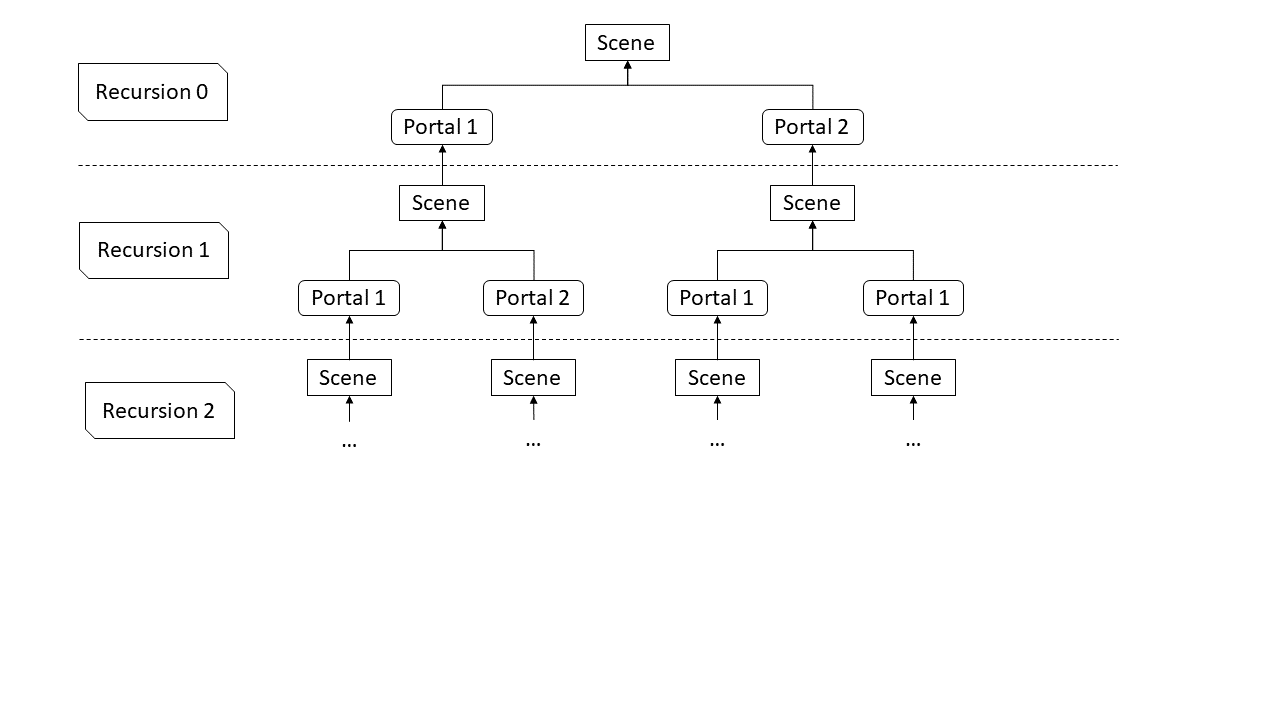
\includegraphics[width=\linewidth]{images/rendertree.png}
	\caption{Render Dependencies}
	\label{fig:rendertree}
\end{figure}


When drawing multiple portals recursively the draw dependencies can be imagined as a tree. Figure \ref{fig:rendertree} shows the dependencies for two portals. In recursion 0 the two portals can only be drawn after the all objects were drawn. Otherwise portals that are occluded by an object might wrongly mark the pixel in the stencil buffer. The two draws of all objects in recursion 1 can only be drawn when their respective portal was already drawn. However, it is not necessary that all portals from recursion 0 were drawn, before objects can be drawn in recursion 1. For example, in recursion 0 portal 1 could be drawn, and the recursion 1 objects that depend on that portal. After this portal 2 from recursion 0 can be drawn.

There are two approaches on the drawing order: depth first or breadth first. In depth first the contents of portal 1 in recursion 0 would be fully complete, before it begins drawing the contents of portal 2 in recursion 0. This has the advantage of needing just a small amount of different values to mark a pixel. Going down the tree a different value can be used for each recursion. When going up that value is not needed anymore and can be recyled. However, the implementation must make sure that no unneeded value remains in the stencil buffer. A downside is, that the draws are is fully dependent on each other.

Breath first draws a recursion completely before drawing the next recursion. The amount of different values needed to mark a pixel, scales super linear with the portal count and \gls{recursioncount}. One value is needed of each portal in a recursion. For a scene with two portals, to mark all portals from recursion 1 it at least needs 4 different values, excluding 0. For recursion 2 it needs 8 values. With the stencil buffer usually being limited to 8 bits this can be quickly become a hard limit. However, the advantage is that the depth buffer needs to be cleared less often, only when transitioning between recursions. Additionally, within a recursion there are not dependencies between the multiple draws of objects, as well as the portal draws.

Previous transformative portal implementations used depth first \cite{lowe:2005:technique,lecture:portalProblems}. The implementation presented in this thesis uses breadth first. There are fewer dependencies between the draws, which could be exploited. Additionally similar draws can be grouped, which reduces the amount of render passes. While the amount of stencil values needed scales super linearly, the amount of draws scales super linearly too. The author believes it is more likely that amount of draws will be the limiting factor than running out of values in the stencil buffer.



\subsection{Generating View Matrices}
\label{section:generatingviewmatrices}


As describe in section \ref{section:textursVsStencil} the scene needs to be rendered from the correct view point. When looking through the portal, it must look as if the camera looks directly a the object.

\begin{figure}[H]
	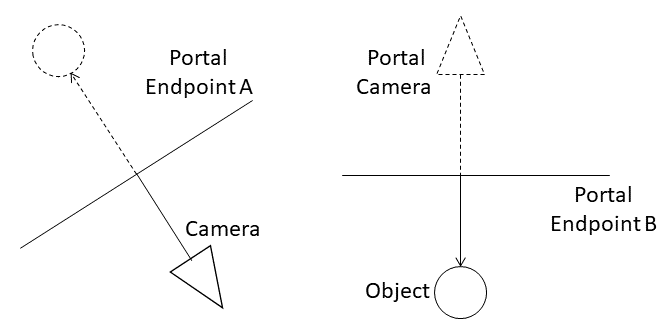
\includegraphics[width=\linewidth]{images/portal.png}
	\caption{A \gls{portalpair} connecting two parts of the world}
	\label{fig:portal}
\end{figure}

Figure \ref{fig:portal} shows the camera looking at endpoint A of a portal pair. It appears as if the dotted circle is in front of the camera. However, the actual circle is somewhere else. Instead of seeing endpoint A, the contents other part of the world is from portal camera's view point are seen.


To move the camera to the correct location the \gls{endpoint}['s] \gls{teleportationmatrix} is be applied to the camera matrix to calucalate the portal camera. Then the portal's \gls{viewmatrix} can be obtained by inverting the portal camera.

%This view point corresponds to the camera's view point teleported by the specific portal's \gls{teleportationmatrix}. As the camera moves the matrices must be calculated every frame.

%\begin{figure}[H]
%	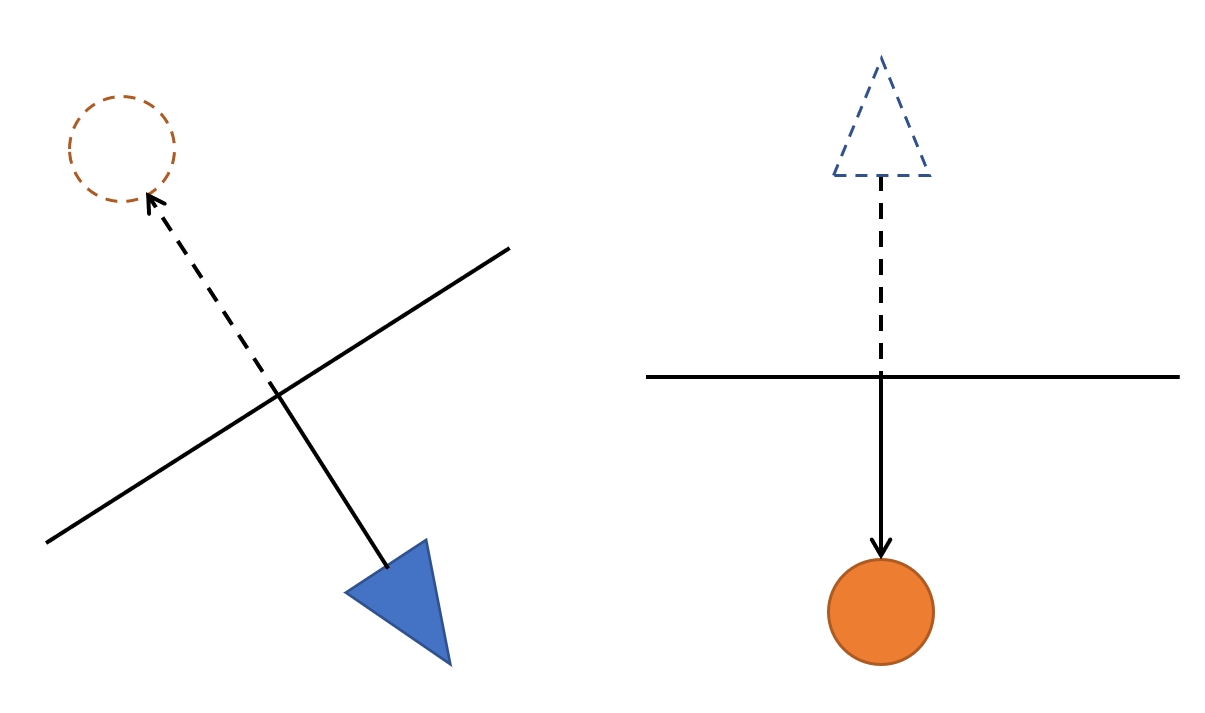
\includegraphics[width=\linewidth]{images/camera_matrices.png}
%	\caption{Portal Camera}
%	\label{fig:cameramatrices}
%\end{figure}

%Figure \ref{fig:cameramatrices} shows two portal endpoints. The blue triangle represents the camera and the orange circle represents an objects. The dotted blue triangle represents the portal view camera.



\subsection{Recursive Portal Matrices}
\label{section:recursivecameramatrices}
The previous section explained how to calculate the camera matrices for each portal for recursion 1. For recursion 2 a the camera's viewpoint must be transform twice, by two sequential applied \glspl{teleportationmatrix}. This needs to be done for every combination of two portals. For recursion 3 this is done for every combination of three portals and so forth. This different combinations of matrices can be seen as a tree. The root is the current camera matrix. An nth child node's matrix is equal to its parent matrix multiplied by the portal n's \gls{teleportationmatrix}. The tree is filled level by level, each level reusing the calculations of the previous level.




The implementations stores this tree of camera matrices in an array. The indices can be found the following way:

\begin{itemize}
	\item $ nth child = current index * portalcount + 1 + n$
	\item $ parent = \lfloor(current index-1)/portal count\rfloor $
\end{itemize}



%%$c_n .. nth child index$
%%$p .. parent index$
%%$i ... curent index$
%%$t ... portal count$

\begin{figure}[h]
	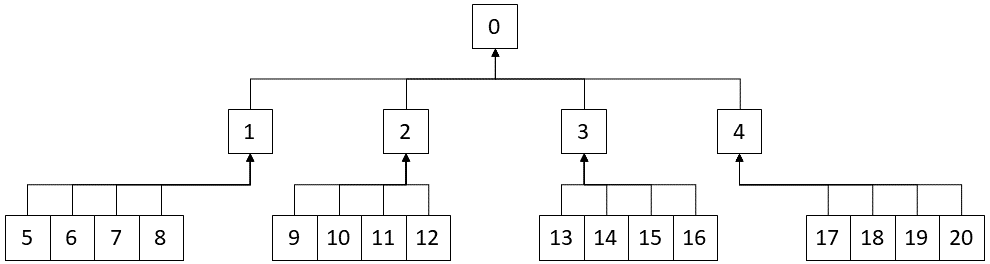
\includegraphics[width=\linewidth]{images/cameraindices.png}
	\caption{Camera Indices}
	\label{fig:cameraindices}
\end{figure}

Figure \ref{fig:cameraindices} shows the indices for 4 portals, with 2 iterations. For example to find the view matrix of Portal 0, seen through Portal 1, we would access the array at index 9. Note that the size of the tree scales exponentially, with the \gls{recursioncount}, as every possible combination of portals needs to be covered. At the end of the calculation of the tree, every matrix of in the tree needs to be inverted.


\subsection{Dual Depth Buffer}

When drawing the scene from the portals view, care must be taken to not draw objects, that are between the camera and other endpoint. In previous works this is often referred to as clipping \cite{lowe:2005:technique}.
\begin{figure}[h]
	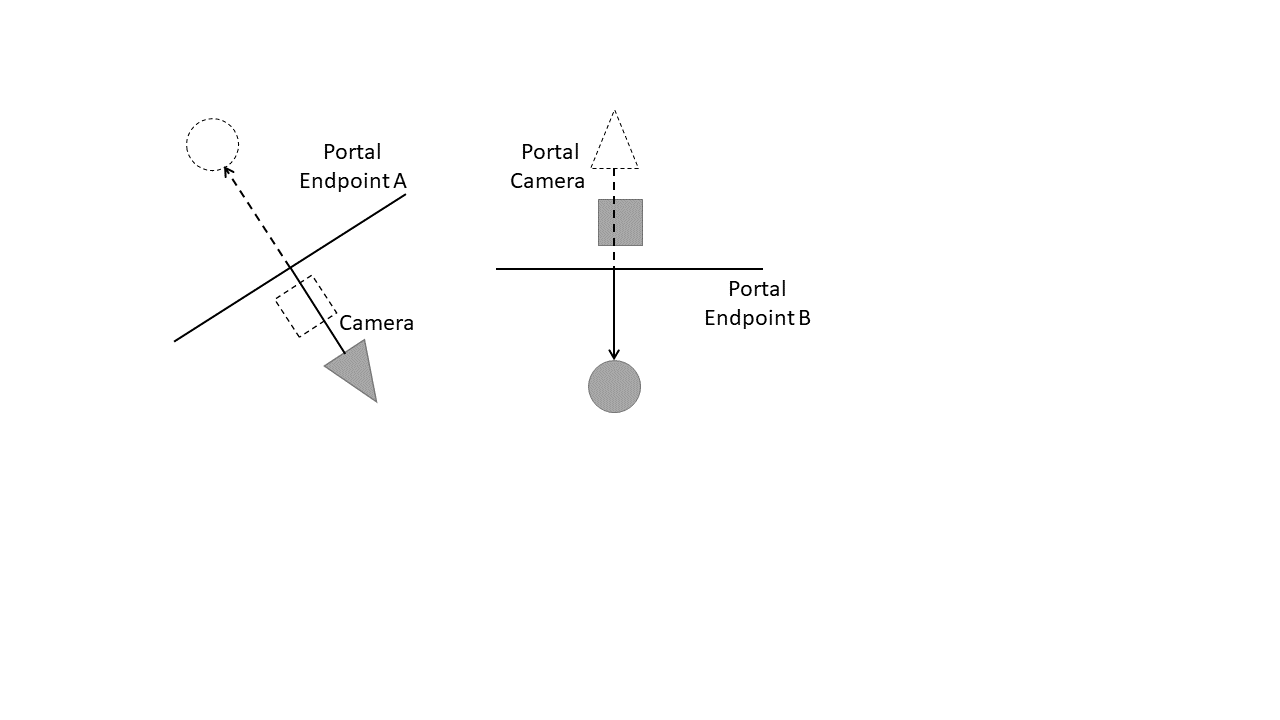
\includegraphics[width=\linewidth]{images/bananajuce.png}
	\caption{Object between portal camera and portal endpoint}
	\label{fig:bananajuce}
\end{figure}

Figure \ref{fig:bananajuce} shows such an example. Without additional techniques the square would be drawn. One possibility would be the use of clip planes. However, this limits a portal's shape to planes. Another solution, which allows for arbitrary portal shapes is to use two depth buffers or dual depth buffer: a near depth buffer and a far depth buffer. The far depth buffer is used to discards fragments with a greater depth value. It is just a regular depth buffer, which is used in almost any rendering system. The near depth buffer discards fragments with a lesser depth value. When rendering the portal its depth is also rendered to the near buffer. The box's depth values from figure \ref{fig:bananajuce} would be greater than the near buffer and its fragments are discarded \cite{lowe:2005:technique, ropinski:2004:real}.

In this implementation the hardware supported depth buffer is used as the far buffer. For the near buffer two buffers in form of colour textures are used, a read near buffer and a write near buffer. This way a old near buffer values can be used, while writing new near buffer values. In the fragment shader, the fragments depth value is compared to the read near buffer. If it is lesser it is manually discarded, with a discard statement in the shader. Whenever the portals are drawn, they not only write the far depth buffer via depth test, but also write to the write near depth buffer via colour output. When the implementation transitions to the next recursion, the write near buffer and read near buffer are swapped.

Dual buffering the near buffer avoids problems with edge cases where one portal occludes another and the portal behind is drawn first. With only one near buffer, the portal behind would set the near buffer to its depth value. The fragments of the portal in front would be discarded, instead of occluding the portal behind.

The read near buffer is a input attachment and the write near buffer is a colour attachment. In recursion 0, no read near buffer test is used.

\subsection{Portal near Z fighting}
\label{section:portalzfighting}
When rendering the contents of one endpoint of a portal pair, the other endpoint would be rendered directly at the same location. They would have the exact same depth value. The other endpoint's fragments would sometimes be discard by the near buffer and sometimes not. This leads to a special case of Z fighting. To avoid this the winding order of a fragment is stored in the near buffer. When the fragments depth value and the near buffer value are nearly equal and winding order is the same, this would be exactly the previously mentioned case and the fragment should be discarded. This is done by increasing the comparison value by some small amount or percentage for same winding orders.

For the prototype the depth values range of 0 to 1, and does not use negative values. This allows the implementation to store the winding order as the sign of the near buffer. Positive depth values indicate front facing and negative depth values indicate back facing. Near Depth comparison is done with the absolute value of the buffer.

\subsection{Stencil Values and compare masks}
\label{section:stencilcomparemasks}

As the implementation uses the breadth first approach, it can not use the stencil increment and decrement technique described in other works \cite{schmalstieg:1999:sewing, lowe:2003:fragment, lecture:portalProblems}. Different values need to be stored and compared against. Directly setting the stencil value can be achieved, by setting a reference value and use the replace stencil operation. However, the stencil reference is also used for the comparison. This means that the implementation must be use the same value for comparison as well as writing. This can be achieved by the use of stencil compare mask and generating stencil values with postfixing.

\begin{figure}[h]
	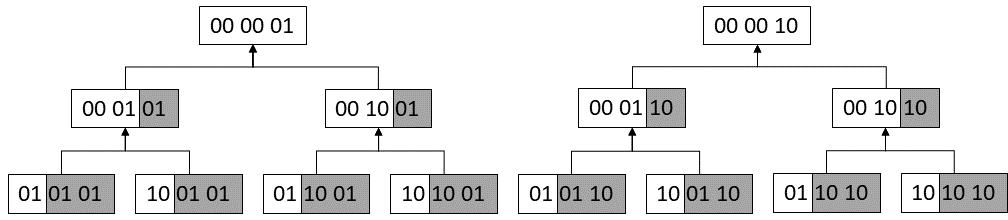
\includegraphics[width=\linewidth]{images/stencilvalues2.png}
	\caption{Compare Mask and Stencil Values}
	\label{fig:stencilvalues}
\end{figure}

Figure \ref{fig:stencilvalues} shows is process with two portals and 6 bits. The grey part is used for comparisons, while the whole value is used to write. The comparison mask of recursion 0 masks out all bits, so the test will always succeed. For two portals recursion 1 mask out all but the last two bits. Notice that the last two bits of  recursion 1's stencil values are the same as their respective parent values. It is important that stencil values start with 1 and not with 0, otherwise they are not distinguishable from their parent values.

This also means that the range of values is one less than representable by the number of bits. This is very significant, as the portals come in pairs. The number of bits needed for two and four portals is one more than normally needed. As the stencil buffer usually only has eight bits, this limits the amount of recursions considerably.



\section{Initial Implementation}
\label{section:intialimplementation}
This section describes the first iteration of the implementation. It uses the specified techniques described in section \ref{section:portaldrawing} and focuses on how those are implemented.


\subsection{Renderpass Setup}
\label{section:renderpasssetup}

The implementation uses just one renderpass, with multiple subpasses. This allows for the use of input attachments and potentially enables the \gls{gpu} driver to optimize. For example many textured are only needed within the renderpass and do not need to be transferred anywhere else.

\begin{figure}[h]
	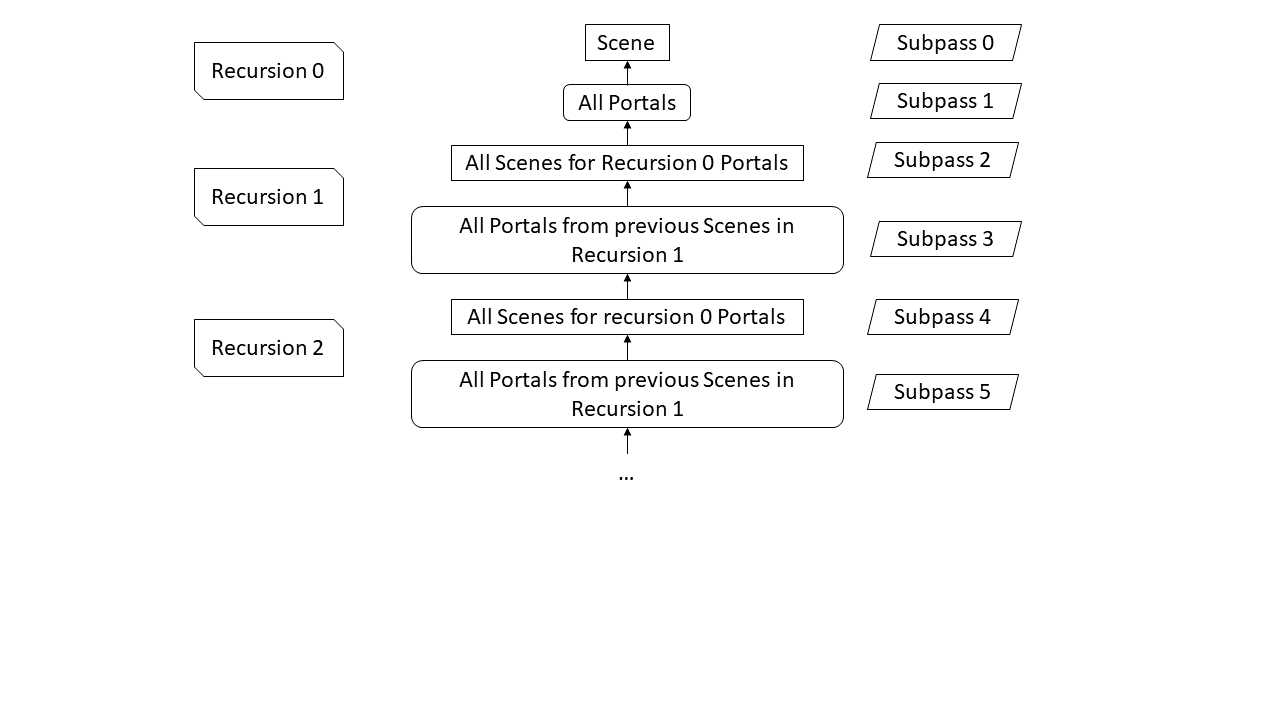
\includegraphics[width=\linewidth]{images/renderpasses.png}
	\caption{Subpasses and work done}
	\label{fig:renderpasses}
\end{figure}


Figure \ref{fig:renderpasses} shows the subpasses, which recursion they belong to and what work is done. Notice that compared to figure \ref{fig:rendertree} object and portal draws are each batched together. Every even subpass is responsible for drawing a objects, while in every odd subpass the portals are drawn. The subpass index divided by two equals the recursion index. 

\begin{figure}[h]
	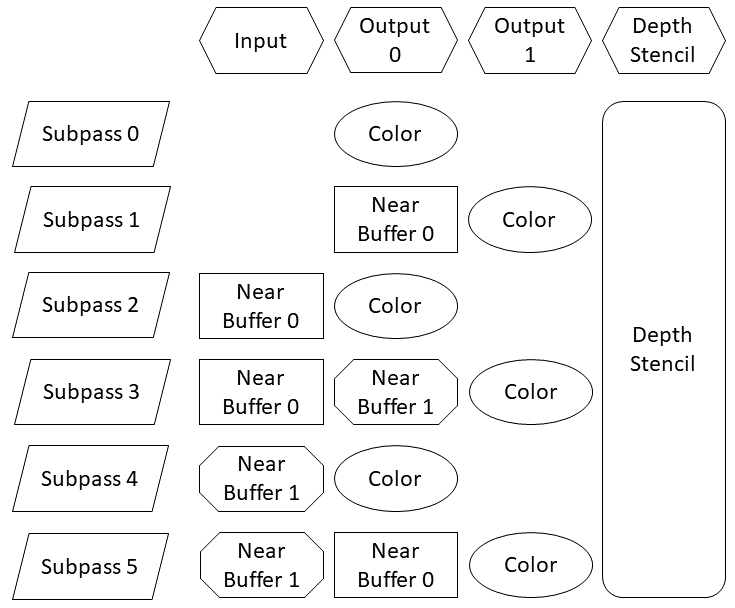
\includegraphics[width=\linewidth]{images/attachmentsetup.png}
	\caption{Attachment Setup}
	\label{fig:attachments}
\end{figure}

Figure \ref{fig:attachments} illustrates the attachments of the individual subpasses for two recursion. Odd subpasses write into the near buffer, which is used as input for the following two subpasses. For a real application portals do not need to write colour so output 1 is not really needed. However, for this implementation it was kept for debugging purposes.
The last subpass does not need to write to the near buffer, as there are not later subpasses which could use it. It is kept for debugging purposes too. The depth stencil attachment is never changed. The colour and depthstencil attachment are cleared at the beginning of the renderpass with VK\_ATTACHMENT\_LOAD\_OP\_CLEAR. Both near buffers use VK\_ATTACHMENT\_LOAD\_OP\_DONT\_CARE. The stencil test ensures that they are only accessed at locations where portals have previously written a value. Each subpass has set a dependency in the fragment shader on the previous subpass' output. The depth part of the depth stencil buffer is cleared after each recursion.


\subsection{Graphic Pipelines}
When rendering the multiple scene one after each other, as well as when rendering the portals, the stencil reference needs to be changed. There are two options how to resolve this problem: either using multiple pipelines or using dynamic pipeline state. For the implementation dynamic pipeline state was used, as the number of graphic pipelines needed would scale super linearly with the amount of portals and recursions. Dynamic state seemed much easier to manage in comparison.

However, the subpass index cannot be dynamic state. Thus even with dynamic stencil references, there must be at least the same amount of graphic pipelines as there are subpasses. If more than one shader is used for rendering scene objects or portals, the amount of graphic pipelines is increased. Each additional shader increase the amount by half of the subpass amount, as it is either only used for portal rendering or only for scene rendering. As there already are different pipelines for the subpasses, each of them can have a different stencil compare mask (see section \ref{section:stencilcomparemasks}). There is no need for dynamic stencil compare masks.

One important aspect is that pipelines for both scene and portal drawing, have face culling disabled. Portals do not have to be watertight and scene object might be transformed in a way that changes winding order. If it can be ensured that there are no teleportation matrices that change winding order, then face culling could be enabled for scene objects. For this implementation it was chosen to support such teleportation matrices.

The individual  graphic pipelines for drawing the scene differ by subpass index and stencil compare mask. This is also true for the graphic pipelines for portal drawing. Additionally, subpass 0 has the stencil test completely disabled, while subpass 1 uses an always succeeding test with VK\_STENCIL\_OP\_REPLACE. Other even subpasses use the stencil compare op VK\_COMPARE\_OP\_EQUAL with VK\_STENCIL\_OP\_KEEP for all test result. Other odd subpasses use VK\_COMPARE\_OP\_EQUAL with VK\_STENCIL\_OP\_REPLACE on stencil and depth test success, otherwise VK\_STENCIL\_OP\_KEEP

\subsection{Shaders}
Vulkan shader module requires the SPIR-V format. The shaders are written using GLSL and are compiled using the GLSL Validator (glslangValidator.exe) from LunarG's Vulkan SDK. All fragment shaders contain the manual check with the near buffer. If it fails the fragment is discarded using the discard statement. However, for subpass 0 and subpass 1 there is no input attachement (see figure \ref{fig:attachments}). For those shaders the check is omitted. To prevent shader redundancies the shader is compiled twice. One of the compilations skips the check using the preprocessor and by command line arguments to the GLSL Validator. As previously mentioned in section \ref{section:renderpasssetup} the portals drawn in the last subpass do not need to store anything in the near buffer. This could also be omitted using conditional compilation. All scene object only have one colour. It is passed via push constants. Additional minimal shading is performed using diffuse only shading with a fixed directional light.

Vertex shaders need to transform the vertices for all the different views. The different view matrices are stored in an \gls{ubo}. The index to access the current view matrix received via push constant. The model matrix is received also via push constant, as it changes per model and it there was still enough space in the push constant. The perspective matrix is passed via \gls{ubo}, as it never changes. Even if it would change than likely at most once per frame. The vertex shaders are the same for all scene draws as well as for all portal draws. No conditional compilation is needed.


The shaders are automatically recompiled after a change, using Visual Studio's Custom Build Tool feature. This enables fast iteration times, and avoids error due to forgetting to compile.

\subsection{Pre draw steps}

At the beginning it is waited on a fence to make sure, that submission of a previous command buffer has already finished. Then the fence is set to the unsignaled state. The camera matrices and perspective matrix are calculated. The result is written the respective \gls{ubo} via memory mapping and memcopy, as they use host visible memory. Their memory is also host coherent, so no explicit flushes are needed.
Then the next image from the swapchain is aquired. A semaphore is passed, which can be waited on before submitting the command buffer.
Lastly the the commandpool for the commandbuffer used for drawing is reset.

\subsection{Filling the command buffer}
The commandbuffer used for drawing was just reset via its commandpool in the pre draw steps. The first command is begin with a parameter indicating that this buffer is used for a one time submit. Then the renderpass is begun. Instanced drawing is not used so instance count is 1 and first instance is 0 for \textit{drawIndexed} calls.

Subpass 0 does not use the stencil buffer, so not reference needs to be set. Before drawing the scene \textit{bindIndexBuffer} and \textit{bindVertexBuffer} is called. All scene object vertices reside in the same buffer, so this only needs to be done once. Then for every object \textit{pushConstants} is called on the command buffer with the object specific push constants and \textit{drawIndexed}. 

To change to subpass 1, first \textit{nextSubpass} is called. Then, similar to supass 0, \textit{bindIndexBuffer} and \textit{bindVertexBuffer} is called.  Then for each portal the coresponding stencil value (see section \ref{section:stencilcomparemasks}) is set dynamically with \textit{setStencilReference}, then \textit{pushConstants} and finally \textit{drawIndexed} is called.

Subsequent even subpasses are similar to subpass 0, but the scene drawn is drawn multiple times. Each time with a different camera matrix id as push constant, as well as calling \textit{setStencilReference} with the different stencil values used in the previous subpass.

Subsequent odd subpasses are similar to subpass 1, but all portals are drawn multiple times. No portal has the same stencil value as any other portal.

In total all objects and all portals are drawn for each possible combination of portals. The amount a draws for each of them is equal to the size of the camera matrices array.


\section{Dynamic Portal Rendering}
One downside of the initial portal rendering strategy was its hard limit of total portals in the scene. It did not matter whether a portal was visible or not, it was always drawn and used up values in the stencil buffer. For two recursions, only 15 or less portals were allowed to exist in the scene. For three recursion only 7 or less, for four recursions only 3 portals were possible. For this reason a new method was derived which is limited by the visible portal count instead of the total portal count. 

When drawing a portal, it uses a stencil value depending on the number of visible portals drawn before it, instead of using a fixed value. However, this also means that the right camera index cannot be known before submitting.


\subsection{View Matrix Selection}
\label{section:viewmatrixselection}
Except for subpass 0 and subpass 1, it is not known which camera index to access, as this depends on what portals were drawn previously. This problem is solved with an indirection.

\begin{figure}[h]
	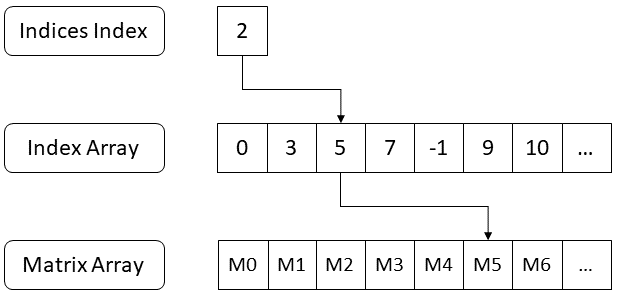
\includegraphics[width=\linewidth]{images/viewmatrixindirection.png}
	\caption{View Matrix Indirection}
	\label{fig:viewmatrixindirection}
\end{figure}

Figure \ref{fig:viewmatrixindirection} shows an example how this works. Instead of receiving the index for the view matrix, an \textit{indices index} is received. The \textit{indices index} is used to access an element in an \textit{index array}. This element's value is the actual index, which is then used to find the correct view matrix in the \textit{matrix array}.

Sometimes there are less visible portals than the maximum count. This can not be known before submitting the command buffer. The draw commands for elements with non existing portals are still recorded in the command buffer. This implementation uses a special value -1 in the \textit{index array} to indicate such a case. It is an invalid index. The value of the view matrix index is the same for every vertex shader invocation of a mesh, as it depends on a push constant value. When encountering and invalid index as view matrix index, the vertex shader sets \textit{gl\_Position} to a fixed position. Every vertex of each triangle of an object, will have the same position. This results in all triangles being degenerate and they are culled \cite{khronos:vulkan:spec1.1}.

\begin{lstlisting}[caption={View Matrix Selection}, label=listing:viewmatrixselection]
// shader.vert
#version 450

...

layout(push_constant) uniform PushConstant {	
	mat4 model;
	int viewMatrixIndicesIndex
	...
} pc;

layout(set = 1, binding = 0) uniform GlobalRenderData {
	mat4 proj;
} u_grd;

layout(set = 2, binding = 0) uniform CameraMats
{
	mat4 mats[maxCameraMatCount];
} u_cMats;

layout(set = 4, binding = 0) buffer ViewMatIndices {
	int vIndices[];
} vi;

layout(location = 0) in vec3 inPosition;

const int invalidmatIndex = -1;

void main()
{
	int viewMatIndex = pc.viewMatrixIndicesIndex == 0 ? 
		0 : vi.vIndices[pc.viewMatrixIndicesIndex];
	
	if(viewMatIndex != invalidmatIndex)
	{
		gl_Position = u_grd.proj * u_cMats.mats[viewMatIndex]
		 * pc.model * vec4(inPosition, 1.0);
	}
	else
	{
		// invalid index, create degenerate triangles
		// by setting every vertex to the same value
		gl_Position = vec4(1);
	}
	...
}

\end{lstlisting}

Listing \ref{listing:viewmatrixselection} shows the code of the vertex shader. Note that if the indices index is 0, it must be recursion 0. 0 can then be used as index for the camera matrices. This is convenient when filling the index buffer later.

\subsection{Properties of the Index Array}
\label{section:indexarrayproperties}

The implementation allows the maximum visible portal count to differ for each recursion. This is useful, as in recursion 0 the draw area is the whole screen, resulting in more visible portals. The contents within portals cover much less screen space, so it is less likely that portals can been seen within them. For each recursion the screen space which is drawn will get even smaller. This means recursion 0 will likely need the most visible portals, while the next recursions will need less and less visible portals.

\begin{figure}[h]
	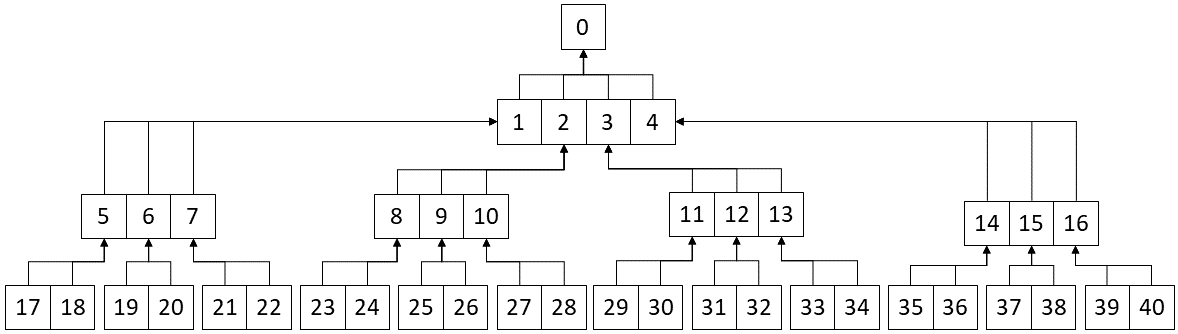
\includegraphics[width=\linewidth]{images/indexarray.png}
	\caption{Index array as tree for 4-3-2 visible portals}
	\label{fig:indexarray}
\end{figure}

Just as the view matrix array, the indices array is also a tree. However, due to the different amounts of visible portals for different recursions, it has a different amount of children in each level. Figure \ref{fig:indexarray} illustrates the connections between child and parent elements. The shown tree supports 3 recursions. The visible portal count for the first recursion is four, for the second it is three and the third recursion it is two. The tree has one root. Each elements child count corresponds to its level in the tree.

The following terms are used for index calculation formulas:
\begin{itemize}
	\item $L_n$ ... the nth level,
	\item $LC_n$ ... the element count of the nth level
	\item $LF_n$ ... the index of the first element of the nth level
	\item $LDC_n$ ... the number of direct child nodes for each element in the nth level. 
	\item $L_nE_i$ ... the index of the i-th element in the nth-level
	\item $L_nE_iC_k$ ... the index of the k-th child of the i-th element in the n-th level 
\end{itemize}

The following formulas can be used to calculate indices:

\begin{itemize}
	\item $LC_0 = 1$
	\item $LC_n = LC_{n-1} * LDC_{n-1}$
	\item $LF_0 = 0$
	\item $LF_n = LC_{n-1} + LF_{n-1}$
	\item $L_nE_iC_k = LF_{n+1} + LDC_{n} * i + k$
\end{itemize}

For every recursion the whole corresponding level of the index array tree is traversed, drawing each object and portal a total of $LC_n$ times. Using figure \ref{fig:indexarray} as example, every object and portal in recursion 0 is drawn 1 time. For recursion 1 is is 4 times, for recursion 2 its is 12 times. And Finally for the last recursion, recursion 3, everything is drawn 24 times. In total 41 draws would be issued for every object and portal.

\subsection{Filling the Index Array}
For the indirection from the previous section to work, the index array must be filled with correct values. Before starting to record draw commands, the index array is filled with an invalid index value by calling \textit{fillBuffer}. Listing \ref{listing:indicesindexcalculation} shows the algorithm used by the fragment shader to calculate and set the individual index array elements.

\begin{lstlisting}[caption={Calculating Indices Index}, label=listing:indicesindexcalculation]
// shader.vert
#version 450
...
layout(push_constant) uniform PushConstant {	
	int viewMatrixIndicesIndex;
	int maxVisiblePortalCount;
	int portalIndex;
	int maxPortalCount;
	int nextLevelStartIndex;
	int portalGroupIndex;
	...

} pc;

layout(set = 4, binding = 0) buffer ViewMatIndices {
	int vIndices[];
} vi;

void main()
{
	...
	int previousVisiblePortalCount = ...
	
	if(previousVisiblePortalCount < pc.maxVisiblePortalCount)
	{
		int currentViewMatIndex = pc.viewMatrixIndicesIndex == 0 ? 
			0 : vi.vIndices[pc.viewMatrixIndicesIndex];
		
		int firstPortalViewIndex = 1 +
			(currentViewMatIndex * pc.maxPortalCount);
		
		int currentPortalViewIndex = firstPortalViewIndex +
			pc.portalIndex;
		
		int firstViewIndicesIndex = pc.nextLevelStartIndex +
			(pc.portalGroupIndex * pc.maxVisiblePortalCount);
			
		int viewIndicesIndex = firstViewIndicesIndex +
			previousVisiblePortalCount;
			
		atomicCompSwap(vi.vIndices[viewIndicesIndex], -1, currentPortalViewIndex);
	}
	...	
}

\end{lstlisting}

In each portals fragment shader the previous visible portal count is calculated. How this is done will be explained in the next section. It is then compared with the maximum visible portal count. If it the previous visible portal count is higher or equal to the maximum visible portal count the index array is not touched by the shader.

If the previous visible portal count is less then the index for writing is calculated using $L_nE_iC_k = LF_{n+1} + LDC_{n} * i + k$ (see section \ref{section:indexarrayproperties}). $LF_{n+1}$ is provided by via push constant and is the same for the whole recursion.  $LDC_{n}$ is also the maximum visible portal count, which was used for the previous check. It is provided via push constant and also stays the same for the whole recursion. $i$ is equal to the number of previous \glspl{portalset} for that recursion. This value will be referred as the \gls{portalsetid}, and is unique within for each draw of a \gls{portalset} in a recursion. It is provided via push constant. $k$ is equal to the number of previous visible portals, that was just calculated.

Now that the index for the element in the index array that should be written to has been calculated, the shader needs to write the right value to it. Using the formula  $ nth child = current index * portalcount + 1 + portalId$ from section \ref{section:recursivecameramatrices} the view index can be calculated.  $currentindex$ was the index used in the vertex shader to access the right view matrix. The $portalcount$ is passed via push constants. $n$ is equal to a portal's \gls{portalid} and passed via push constants.

Every fragment shader invocation will either write the same value or write nothing at all. If no value was written to an index array element, its value will be the invalid index value. For the last portal iteration a visible portal count of 0 is passed. This is an indicator that it is the last recursion. This prevents the portals from writing past the end of the index array.

\subsection{Visible Portal Number algorithm}
\label{section:visibleportalcount}
A portal is visible if at least one fragment of it was drawn. One commonly way of finding out if fragments were drawn are occlusion queries. Reading back the result of a occlusion to the \gls{cpu}, was deemed too slow. Although Vulkan also supports copying the result to a buffer by calling \textit{copyQueryPoolResults} on a command buffer, this is only possible outside of a renderpass. For this reason a different way of finding out, how many different portals are visible was derived.

The algorithm uses an helper array with integer elements and each drawn \gls{portalset} exclusively owns a range within it. No other group may read from or write to that range. This range is called \textit{Helper Range}. The first index of the range is called \textit{First Helper Index}. The size of the range is equal to the \gls{portalcount}. Each portal in a group has an element within range, where it has exclusive write access. It is called \textit{Current Helper Element}. The index to that element is called \textit{Current Helper Index}. Before starting to draw the each element of the helper array is set to 0.

\begin{lstlisting}[caption={Calculate Previous Visible Portals}, label=listing:previousvisibleportals]
// portal.frag
#version 450
#extension GL_ARB_shader_stencil_export : enable

...
layout(push_constant) uniform PushConstant {	
	int maxVisiblePortalCount;
	int portalIndex;
	...
} pc;

layout(set = 5, binding = 0) buffer PortalIndexHelper {
	int indices[];
} pih;

void main()
{
	...
	int previousVisiblePortalCount = 0;
	int currentHelperIndex = pc.firstHelperIndex + pc.portalIndex;
	
	// stop at currentHelperIndex as we are not allowed to read it
	// and the following elements were not written yet
	for(int i = pc.firstHelperIndex; i < currentHelperIndex; ++i)
	{
		previousVisiblePortalCount += (pih.indices[i]) == 0 ? 0 : 1;
	}
	
	if(previousVisiblePortalCount < pc.maxVisiblePortalCount)
	{
		atomicCompSwap(pih.indices[i], 0, previousVisiblePortalCount);
		...
	}
	...
}
\end{lstlisting}

Listing \ref{listing:previousvisibleportals} shows the fragment shader algorithm. Each portal's fragment shader iterates from the \textit{First Helper Element} to the element before the \textit{Current Helper Element}. It increases a counter, each time the element is not zero. This count is equal to the number of previous visible portals and can be used for future calculations. Before drawing the next portal, a pipeline barrier is inserted, so that the writes of current portal's fragment shader are visible to the next portal's fragment shader.

This algorithm makes use of the property that if the fragment shader is never invoked, it will never write a value to its \textit{Current Helper Element}. If multiple shader invocations write the same non-zero value to the \textit{Current Helper Element} there will be that value, no matter how many invocation have written to it.
Thus if at least one fragment shader was invoke for the portal, there will be a non zero value at its position. As the element which is written to, is not read, the write does not influence the other shader invocations. The iteration does not need to continue after \textit{Current Helper Element}, as these values will not have been written yet and will always be 0.

The written value may can be any non-zero value, but writing the previous visible portal count allowed for easier debugging during the creation of the implementation.

\subsection{Properties of the Helper array}
\label{section:helperarrayproperties}
The helper array and index array have a similar structure. For every element in the index array the \gls{portalset} is drawn. During the draw of one \gls{portalset} \gls{portalcount} elements in the index helper array are used. For the final last draw no indices need to be calculated, as nothing will be drawn after it. Thus the element count of the index helper array is equal to the element count of the index array, without its last level, times the \gls{portalcount}.

\begin{figure}[h]
	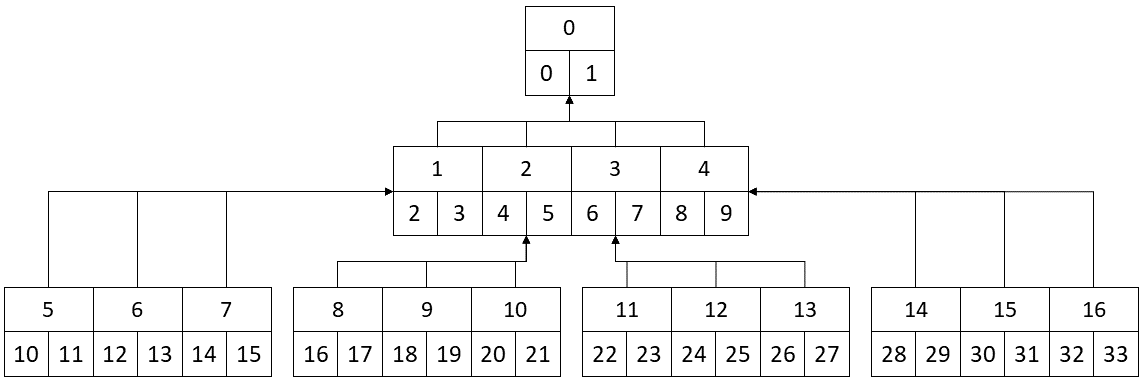
\includegraphics[width=\linewidth]{images/helperarray.png}
	\caption{Helper array as tree for 4-3-2 visible portals, with \gls{portalcount} of 2}
	\label{fig:helperarray}
\end{figure}

Figure \ref{fig:helperarray} shows the helper array as tree, with a \gls{portalcount} of 2. It uses the same recursion count and visible portal count as the index array of figure \ref{fig:indexarray}. The top number in the bigger rectangle corresponds to the index helper tree for easier comparison. Notice that the first index of the actual elements in the bottom boxes is equal to are the top number times the \gls{portalcount}. This first index corresponds to the individual \textit{First Helper Indices}. The same formulas as described in section \ref{section:indexarrayproperties} can be used to calculate those indices. They first need to be divided by the \gls{portalcount}, then used in the formula and the result multiplied by \gls{portalcount}.


\subsection{Calculating the Stencil Reference}
Before drawing it is not known how which and how many portals are actually visible. The stencil value cannot be set dynamically when recording the command buffer. Instead the stencil reference is calculated in the shader and set via the Vulkan extension VK\_EXT\_shader\_stencil\_export. As this is an extension this feature is not supported on every \gls{gpu}.

\begin{lstlisting}[caption={Calculate Stencil Reference in Shader}, label=listing:stencilcalculation]
// portal.frag
#version 450
#extension GL_ARB_shader_stencil_export : enable

// ...
layout(push_constant) uniform PushConstant {	
	uint parentStencilReference;
	int stencilReferenceBits;
	int maxVisiblePortalCount;
//...
} pc;

out int gl_FragStencilRefARB;

void main()
{
	...
	int previousVisiblePortalCount = ...
	
	if(previousVisiblePortalCount >= pc.maxVisiblePortalCount)
	{
		...
		uint myStencilReference = previousVisiblePortalCount + 1;
		uint stencilReference = pc.parentStencilReference 
		| myStencilReference << pc.stencilReferenceBits;
		gl_FragStencilRefARB = int(stencilReference);
	}	
	...
}
\end{lstlisting}

Listing \ref{listing:stencilcalculation} illustrates the calculation. The current stencil reference is passed via push constants. This value changes per drawn \gls{portalset}. It corresponds to the stencil reference of the visible portals of the previous recursion. The fragment shader calculates the current visible portals and adds 1 to it, as using 0 as stencil reference would lead to ambiguities (see section \ref{section:stencilcomparemasks}). That stencil reference needs to be shifted by the amount of bits used by parent stencil reference and then ORed together. Shifting is done using unsigned types to avoid potential undefined behavior.

\subsection{Atomic Writes to Storage Buffer Objects}
In listing  \ref{listing:indicesindexcalculation} and \ref{listing:previousvisibleportals} \textit{atomicCompSwap} was used to write to the storage buffer objects. This was to avoid potential problems due to race conditions. However, it needs to be investigated if these are actually needed. The written values are never read during the shader invocations of one portal. Before they are read by another portal, there is always a memory and execution barrier. For the implementation the atomic operations were left in, as they did not affect performance.

\section{Dynamic Portal instance rendering}
\label{section:dynamicportalinstancerendering}
Dynamic Portal Rendering shifted the limit from maximum portals in a scene to maximum visible portals, while also improving performance a bit. However, the prototype still had many areas to improve. Every object and portal was drawn many times for all the visible portals and recursion. Additionally, using stencil export significantly reduces the number of devices the implementation can run on. As the fragments tests are happening late, portals that would have been discarded by stencil and depth test still counted as visible. This lead to two changes in the implementation.

Firstly, manual stencil testing was tried out. After seeing no real performance penalty this manual test replaced the old stencil test.

The other change was to batch all draws with instanced rendering. Most changes to the code were transforming transforming the loops. Listing \ref{listing:looptransform} shows the difference in pseudo code.

\begin{lstlisting}[caption={Pseudocode Loop Transformation}, label=listing:looptransform]
// old 
for(int i = 0; i < previousPortalCount; ++i)
{
	commandBuffer.setStencilRefrence(stencilReferences[i]);
	for(int k = 0; k < sceneObjectCount; ++k)
	{
		commandBuffer.pushConstants();
		commandBuffer.drawIndexed(sceneObjects[k], 1);
	}
}

// new
for(int i = 0; i < sceneObjectCount; ++i)
{
	commandBuffer.pushConstants();
	commandBuffer.drawIndexed(sceneObjects[i], previousPortalCount);
}
\end{lstlisting}


Calculating the stencil references can be simplified. Using the same stencil reference to compare and set the stencil buffer is no longer needed. The stencil reference values now increments by one for each instance. In fact the stencil reference value and indices index is the same. The indices index for the first instance is passed via push constants. The shaders can calculate their current \textit{indices index} and stencil reference by adding gl\_InstanceIndex to it.

As push constants cannot change for between drawing instances of drawing an objects, all uses of  \gls{portalsetid} are replaced with gl\_InstanceIndex.

As the portal \gls{portalsetid} determines the \textit{first helper index}, all instance of the drawn portal will use a different range in the helper index array. They do not interfere with each other. As there is no synchronisation needed between the instances they can all use instance drawing and have their draw loop transformed similar to the scene objects. However, pipeline barriers are still needed between drawing different portals.

Changing the code to use instance drawing, resulted in a huge performance improvement. Compared to the previous version, the code was 6 times faster on a particular configuration. Additionally, the manual stencil test allows earlier fragment shader discards, reducing the amount of false visible portals. Furthermore, the stencil export extension is no longer required, so the application can run on a wider range of graphic cards. Finally, the texture used for the manual stencil test can be bigger than a real stencil buffer. This effectively removes a hard limit of the maximum visible portals count and recursion count. Those are now only limited by computation speed.


\section{Portal Collision}
One important aspect of portals is actually moving objects. For this implementation teleporting was implemented only for the camera, as a proof of concept.

\subsection{Collision Detection}
The camera is imagined as an object without volume. Each time the camera is moved a ray cast is performed from the camera's old location to its new location. The ray intersection is first performed against the portals' \glspl{aabb}. For the test a the method described by \textcite{williams:2005:efficient} was used. If the test passes the ray is tested the portals mesh's triangles using the triangle intersection algorithm described by \textcite{moller:2005:fast}.


The triangles and bounding box are store in the model space coordinates. This way only one triangle mesh and bounding boxed needs to be stored for portals using the same model. Before a the ray is tested against bounding box and triangles it needs to be transformed into model space. This is achieved by applying the portal's inverse model matrix to the ray.

\subsection{Collision Response}

After a collision the camera needs to be moved to the correct location. The process is the same as the one used to calculate the view point (see section \ref{section:recursivecameramatrices}). However, this matrix can not be directly applied. The camera's position and rotation are not stored as matrix. And additional matrix was added to the camera object, called \textit{additional transform}.

Whenever the camera's position, rotation or camera matrix is needed, they are first modified by the \textit{additional transform}. \textit{Additional transform} is initially equal to the identity matrix. Whenever portal collision occurs, the \textit{additional transform} is multiplied with portal's teleportation matrix.



\section{Camera Object Rendering}
When looking through a portal the camera should see itself, being represented by a camera model.However, if that model was rendered in recursion 0 the view would be inside that model. The implementation avoids this problem, by only conditionally drawing the camera model. In the first subpass drawing the camera is skipped. It is only drawn for subsequent passes.




\chapter{Analysis}
While section \ref{section:implementation} covered how the prototype was built, this section will first showcase and then analyse it. Measurements will be performed and a special kind of transformative portal will be discussed.

\section{Implementation Showcase}

For testing the implementation a demo scene was built. This section demonstrates multiple recursion as well as the use of arbitrary portals.

\begin{figure}[H]
	\centering
	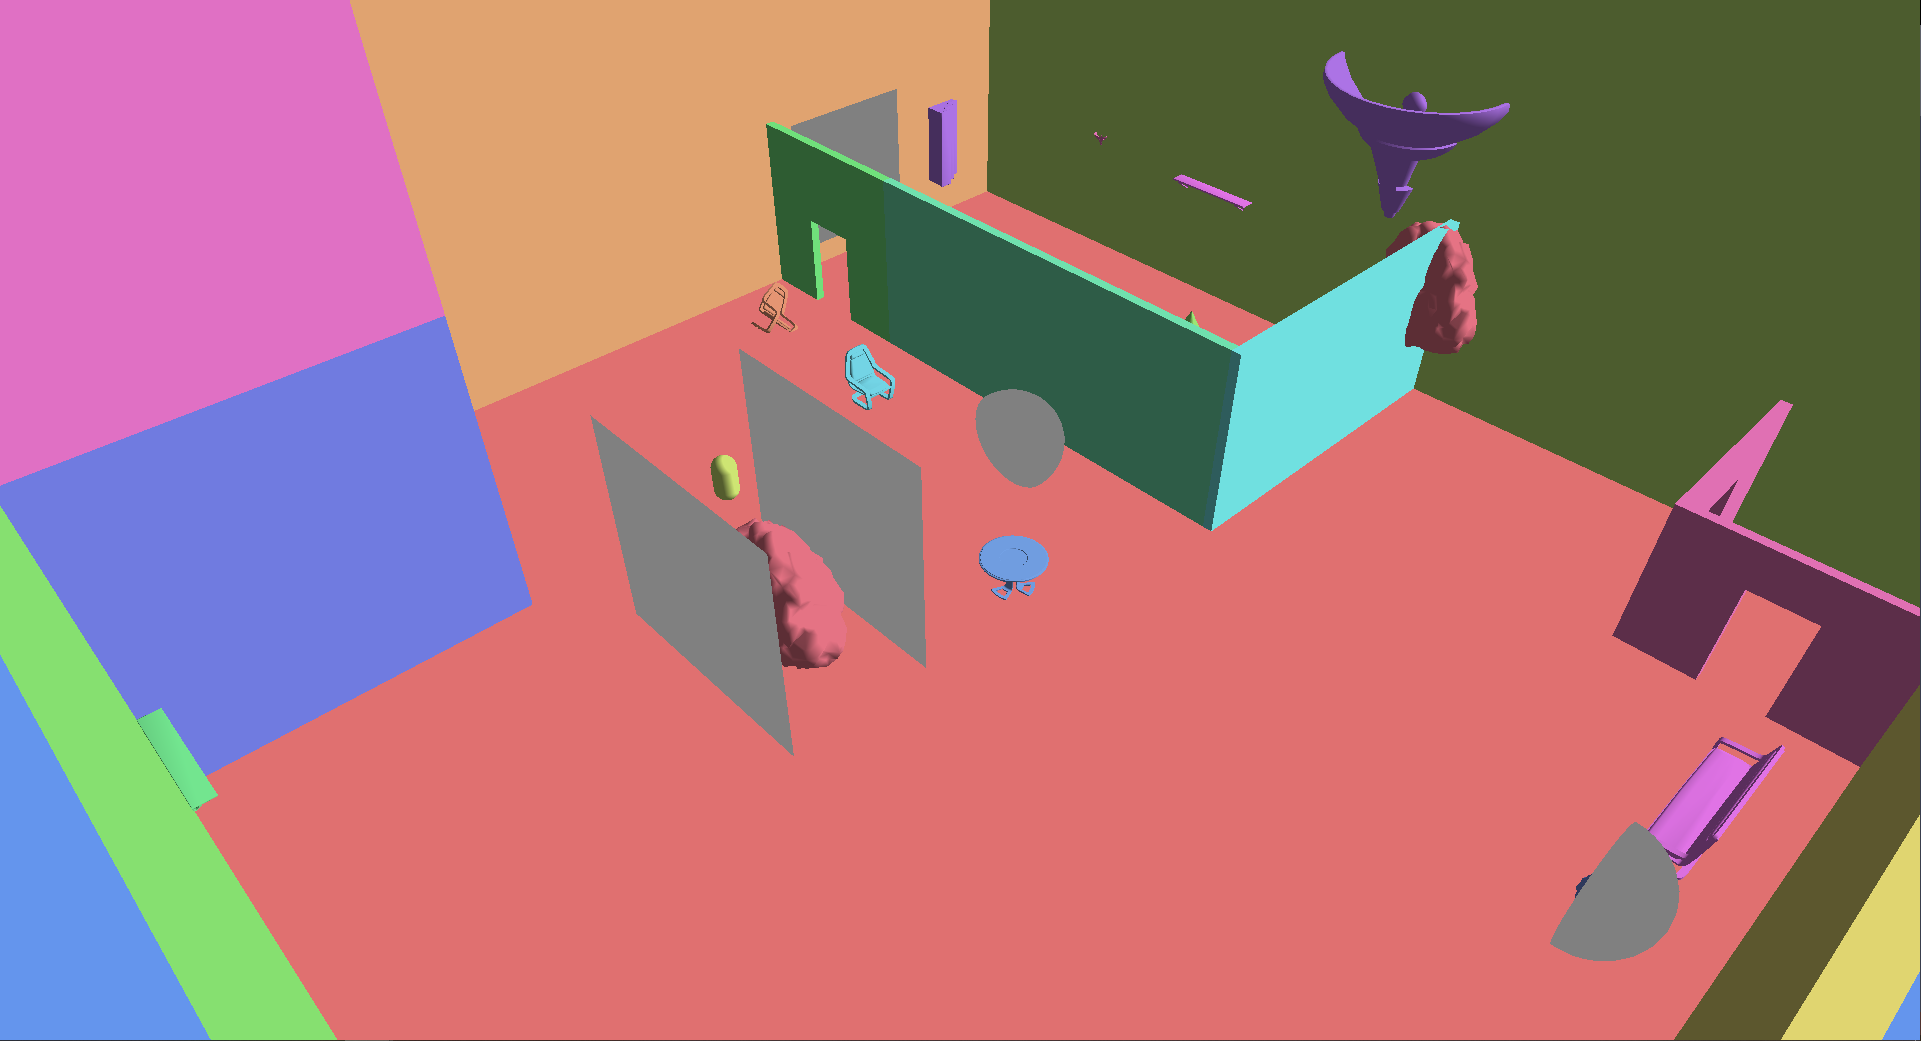
\includegraphics[width=\linewidth]{images/portals.png}
	\caption{Demo scene with no recursions}
	\label{fig:demodisabled}
\end{figure}


Figure \ref{fig:demodisabled} shows a snapshot of the scene. The \gls{recursioncount} was to 0, essentially disabling the portals. They are displayed in grey, which is the colour indicating reaching the maximum recursion count. Note that portals' transform and shape can be completely arbitrary.

\subsection{Recursions}

\begin{figure}[H]
	\centering
	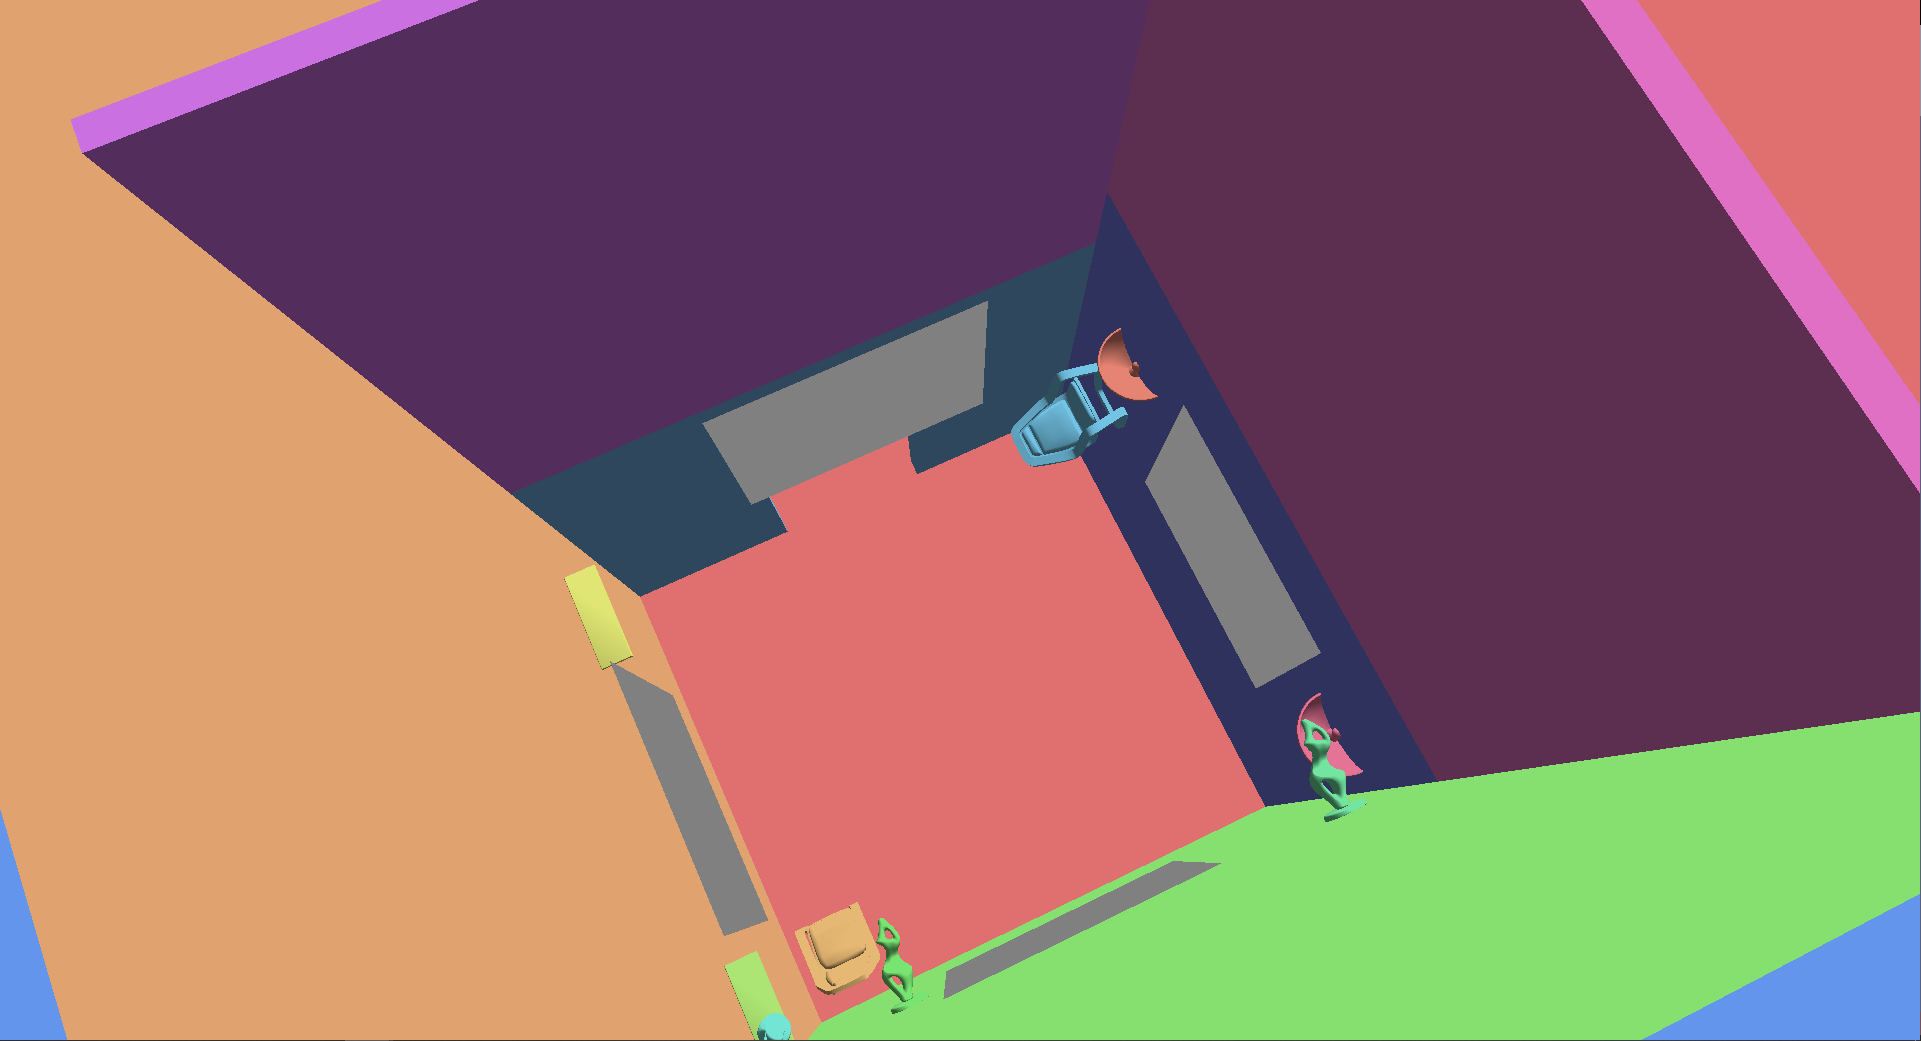
\includegraphics[width=\linewidth]{images/room.png}
	\caption{A room seen from the top, with recursion count 0}
	\label{fig:roomlayout}
\end{figure}

Figure \ref{fig:roomlayout} shows a room within the scene from the top with disabled portals. The top and the left portals form one portal pair, while the bottom an the right portal form another portal pair.

\begin{figure}[H]
	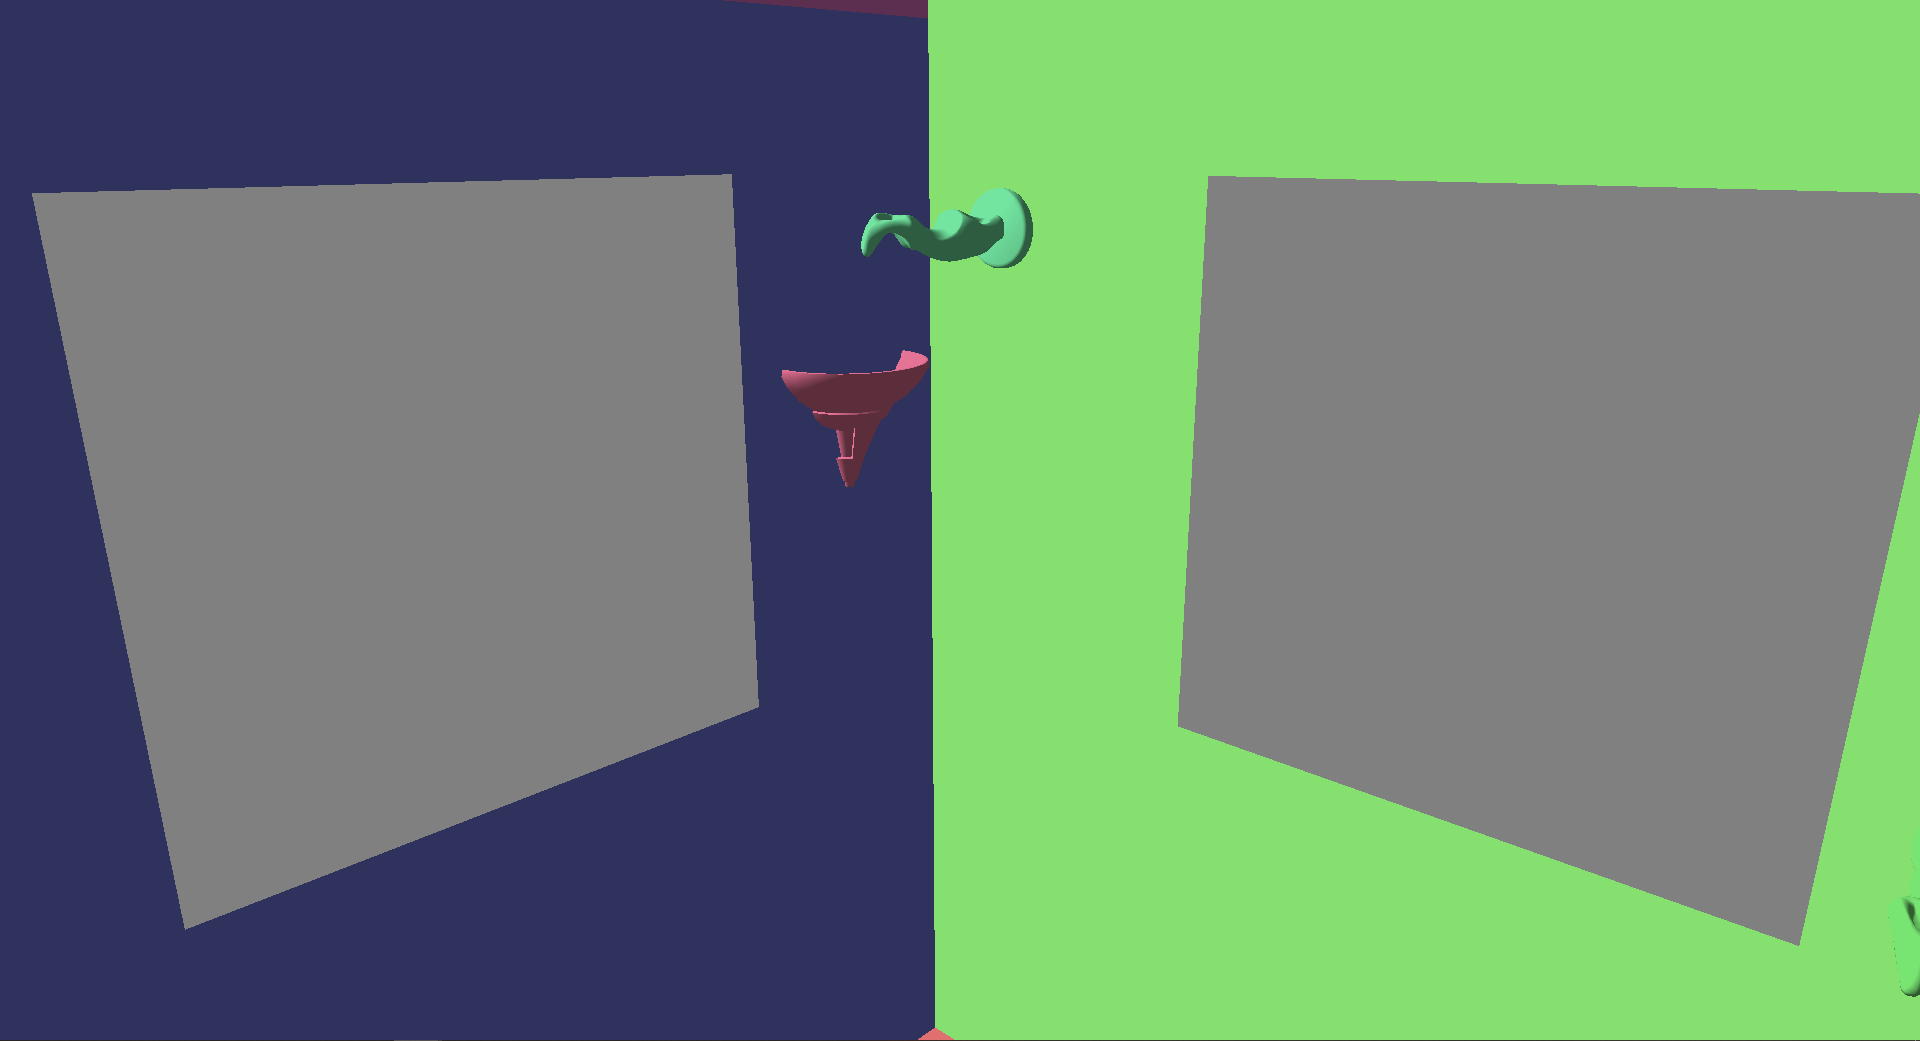
\includegraphics[width=\linewidth]{images/roomportalsr0.png}
	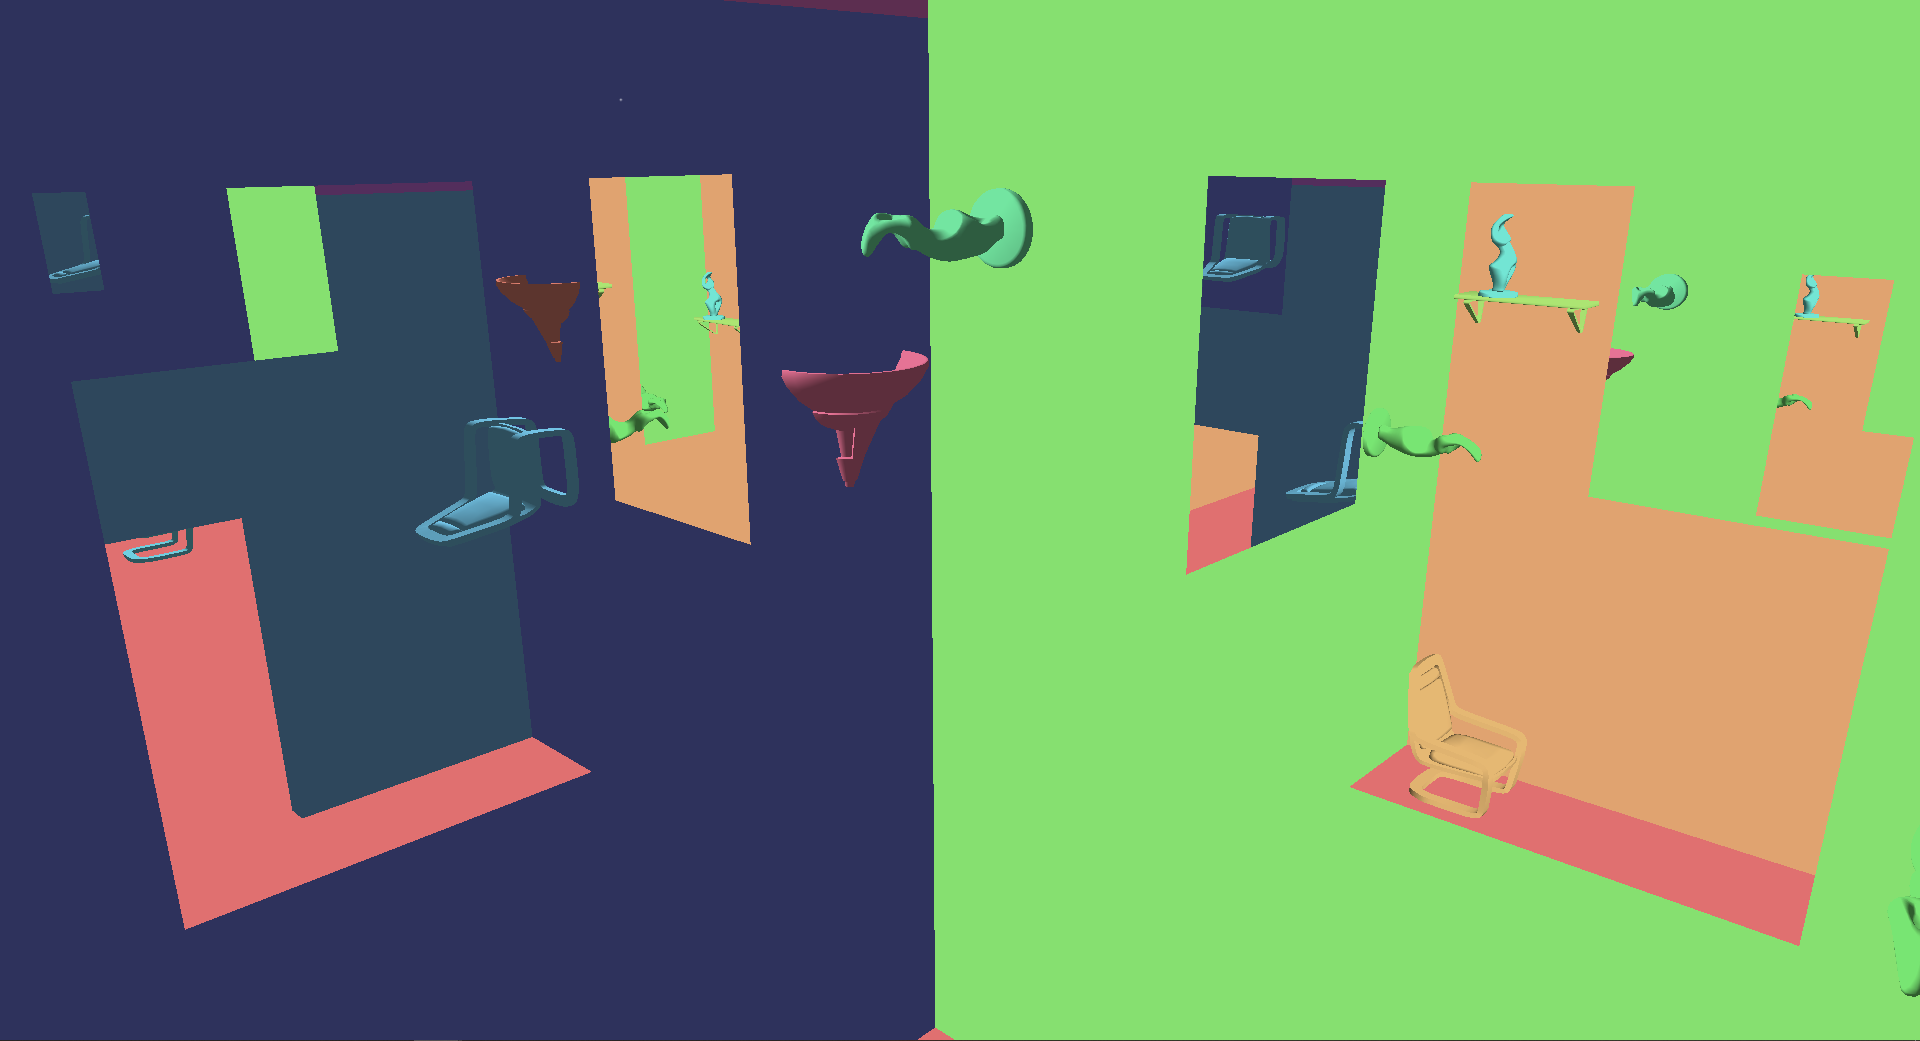
\includegraphics[width=\linewidth]{images/roomportals.png}
	\caption{Another viewpoint of the room.  The top picture is with recursion count of 0, the bottom with a recursion count of 4}
	\label{fig:room}
\end{figure}


Figure \ref{fig:room} shows the same room from figure \ref{fig:roomlayout}, but from a different view point. The top image has a \gls{recursioncount} of 0, while the bottom has a \gls{recursioncount} of 4. Note that the orange and light blue coloured walls cannot be seen without the portals. On the right side multiple recursion can be seen. The green and orange wall are alternating. This indicates that more than one portal pair is involved in the recursion.

\subsection{Non Planar Portals}
\label{section:nonplanar}

This sections showcases portals, that are defined by half spheres. It shows the the implementation works with non planar portals.

\begin{figure}[H]
	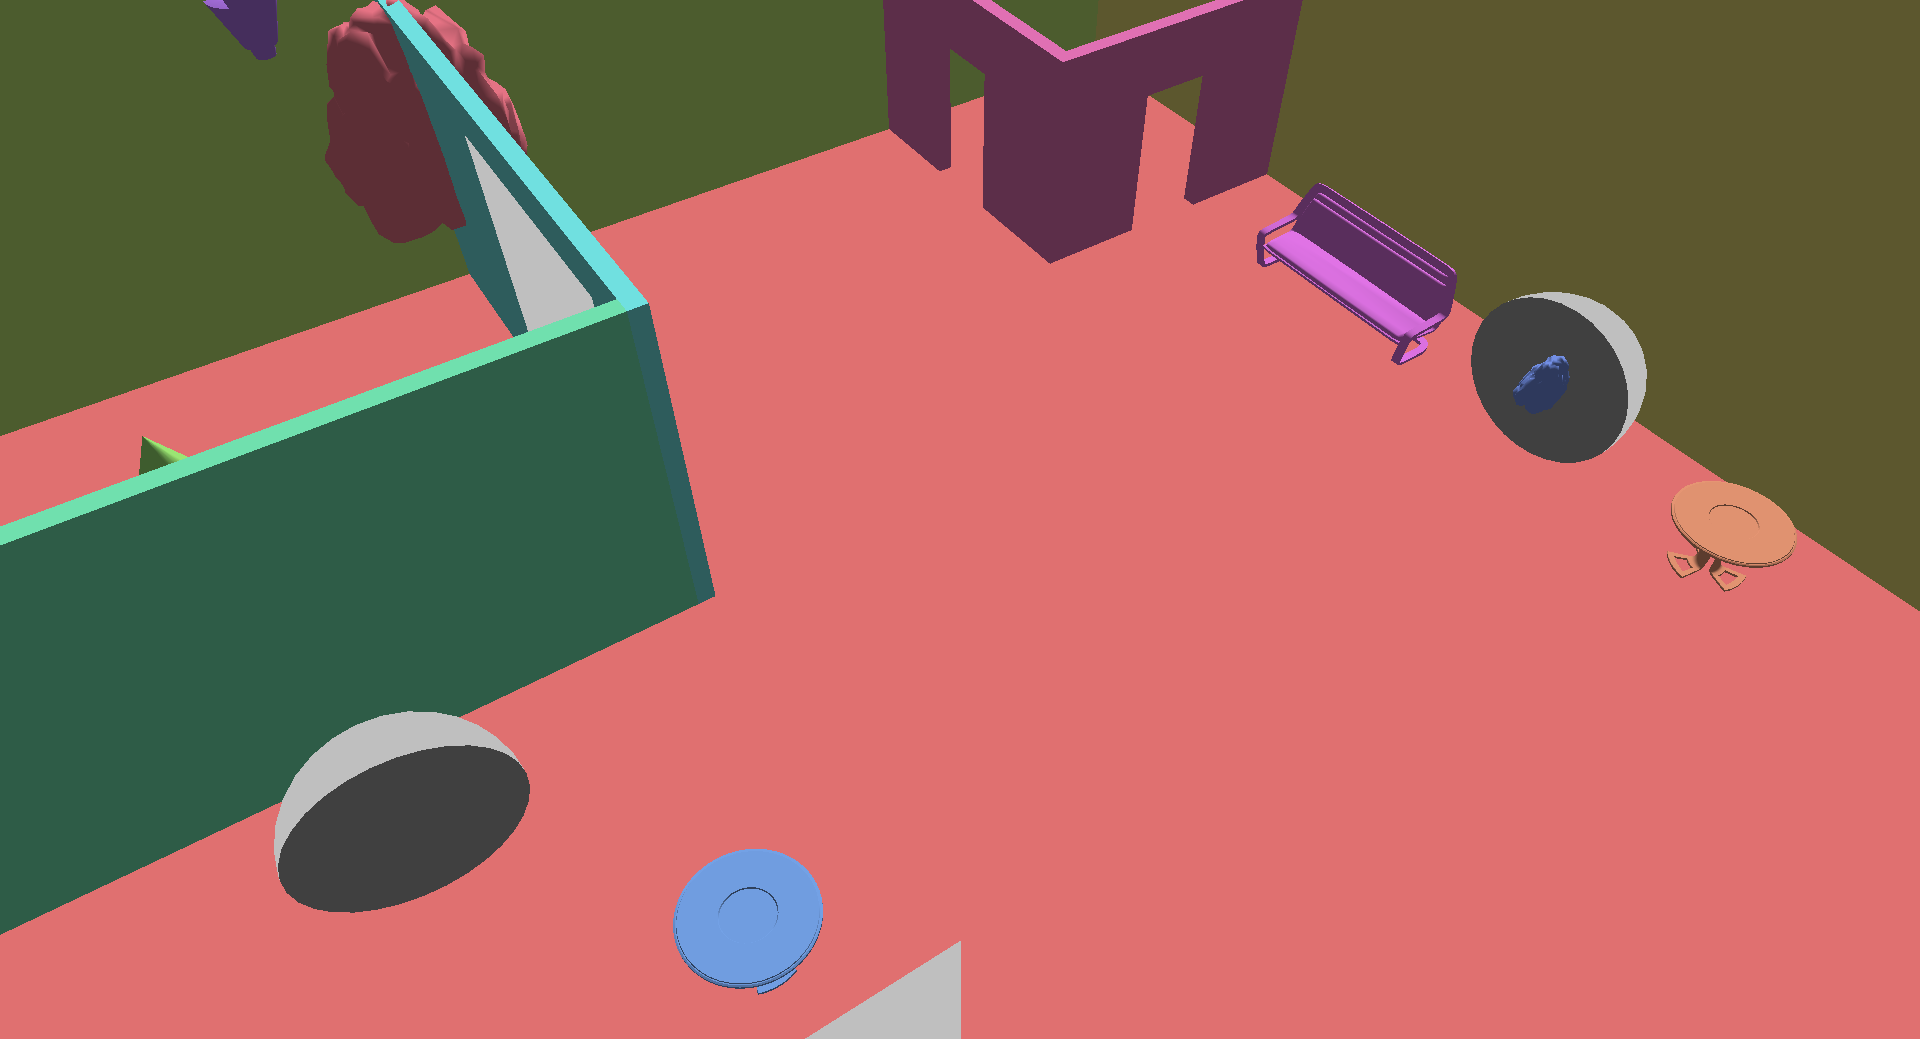
\includegraphics[width=\linewidth]{images/nonplanarlayout.png}
	\caption{The two half sphere portals and their surroundings}
	\label{fig:nonplanarlayout}
\end{figure}

Figure \ref{fig:nonplanarlayout} shows the the two half sphere portals and their surroundings. The half spheres front face are in light grey, while their back faces are in dark grey. Notice that the blue rock on the right side, is inside the half sphere and can be seen through its opening.

\begin{figure}[H]
	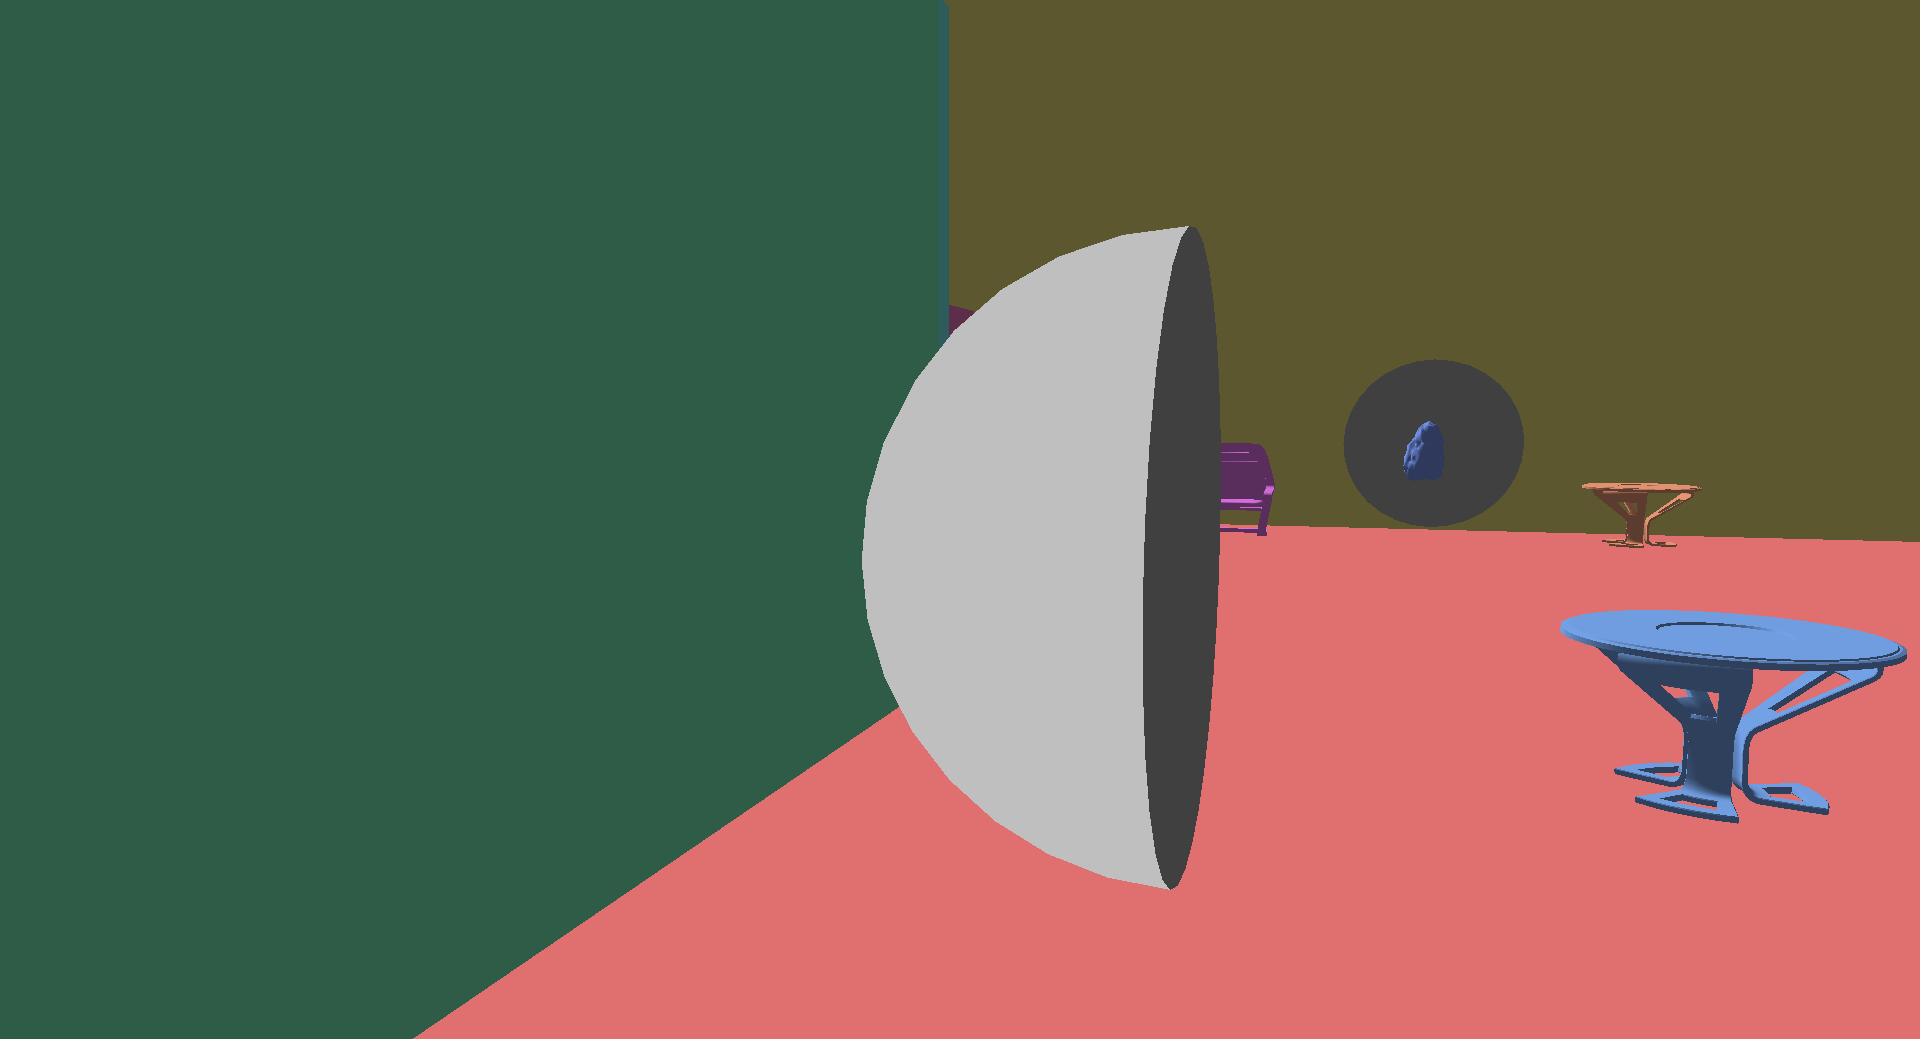
\includegraphics[width=\linewidth]{images/NonPlanarR0.png}
	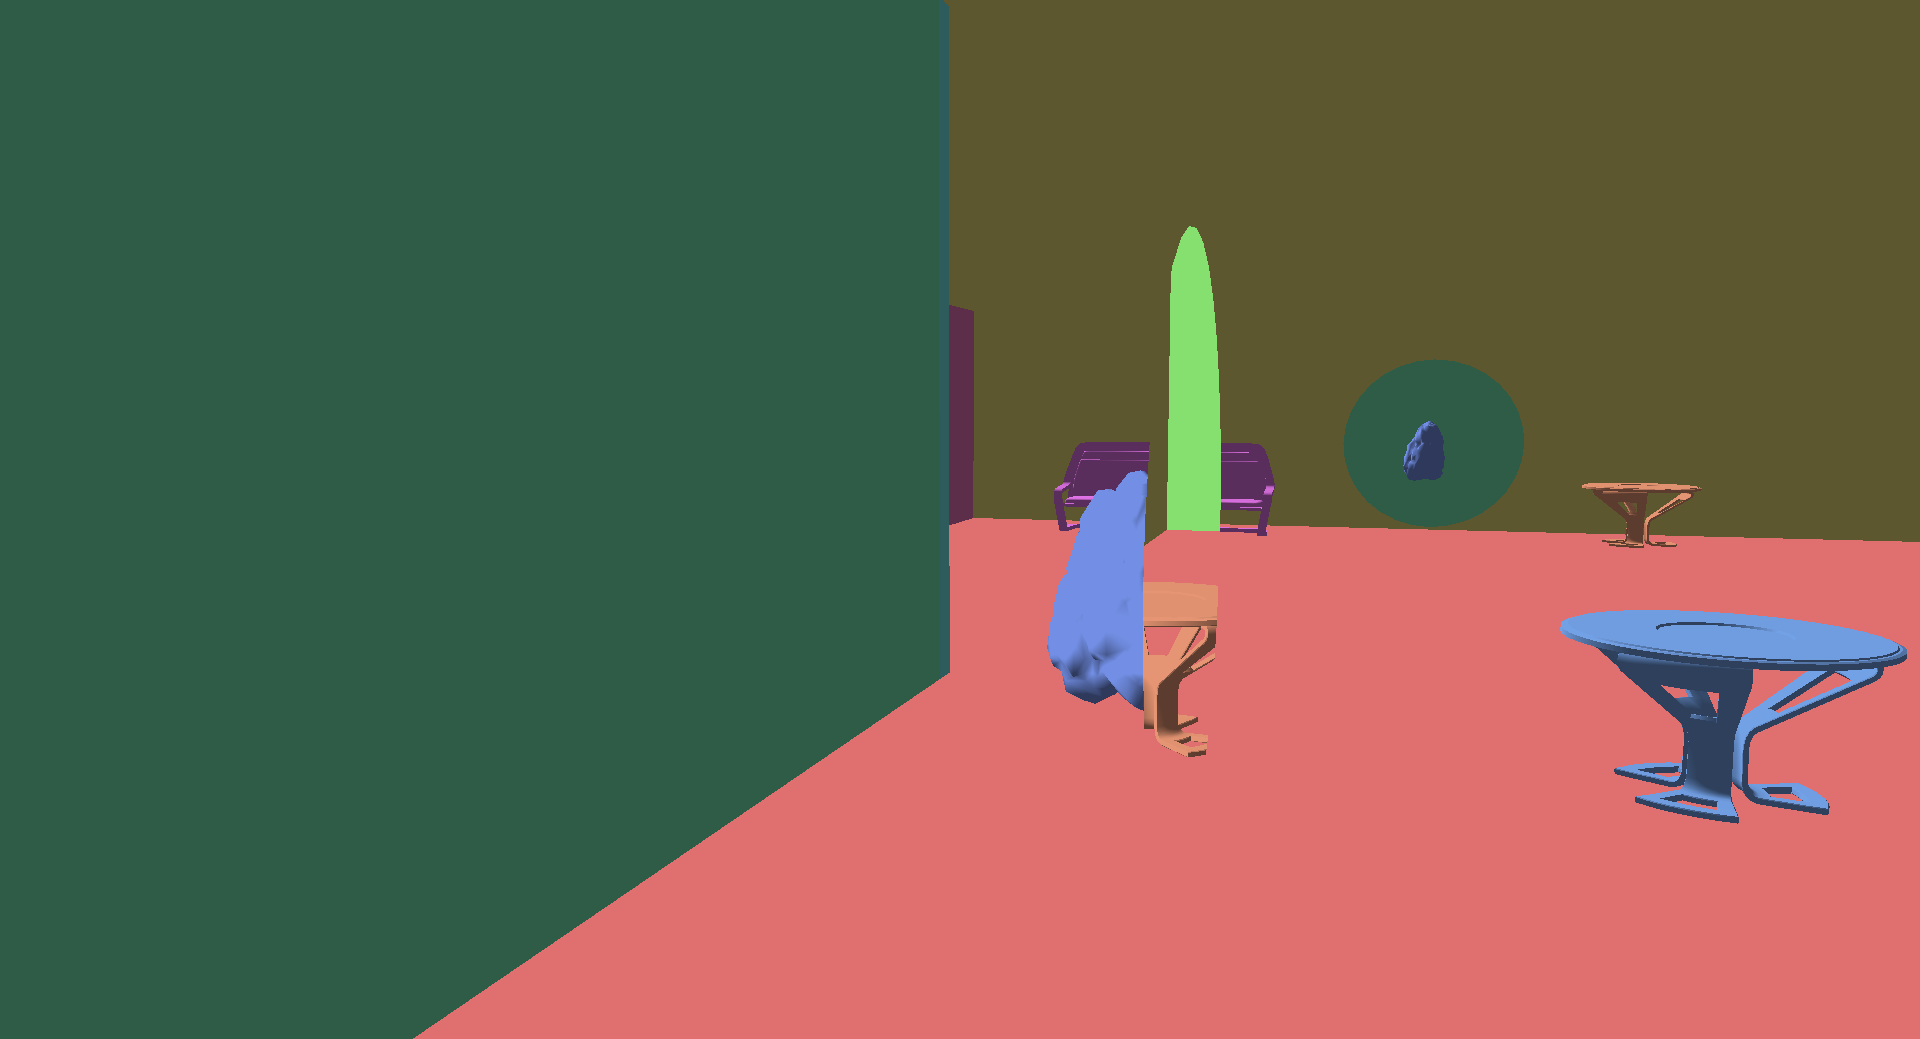
\includegraphics[width=\linewidth]{images/nonplanar.png}
	\caption{The two half sphere portals. The top picture is with recursion count of 0, the bottom with a recursion count of 4}
	\label{fig:nonplanar}
\end{figure}

Figure \ref{fig:nonplanar} shows the same two half sphere portals from another viewpoint. The top picture is with recursion count of 0, the bottom with a recursion count of 4. In this picture the light grey colour not only indicates the portals front face. Additionally, for this case the light grey colour indicates at which pixels two recursions take place. At the dark grey pixels there is only one recursion. The front half sphere portal will be referred as \gls{endpoint} A and the back half sphere portals as \gls{endpoint} B.

Notice that in the bottom picture more parts of pink bench behind the \gls{endpoint} A are visible. The two portal recursions cancel each other out. Additionally, the blue rock which is inside \gls{endpoint} B can be seen. The contents of \gls{endpoint} A and B appear swapped. When looking through the hole in \gls{endpoint} A, the orange table next to \gls{endpoint} B can be seen. Inside \gls{endpoint} B a green colour can be seen, which is the same colour as the one from the wall next to \gls{endpoint} A

\section{Implementation Performance}
\label{section:performancemeasurement}

This sections covers performance measurements. With these the suitability for real time applications can be concluded. Additionally bottlenecks can be discovered, providing insights on how the prototype can be improved in the future.

\subsection{Measuring method}
All tests are run on the same machine. It runs on Microsoft Windows 10 Education (10.0.18362). It uses \gls{gpu} is AMD Ryzen 7 1700 as \gls{gpu} and the Radeon RX 570.

In this test measures the time taken to render one frame. This includes the time the \gls{cpu} needs to prepare the data for the \gls{gpu} (e.g. calculating camera matrices) as well as recording the command buffer. The time is measure in milliseconds using C++'s chrono library. The time is measured for 128 consecutive frames. The average, median, minimum and maximum time of the measured times are printed to the console.


The measured milliseconds differ depending on the current view point and looking direction. Multiple viewpoints were measured. Multiple recursion counts and maximum visible portals are measured. The recursion are note in the form  X-Y-Z, where X corresponds to the maximum visible portals in recursion 0, Y to maximum visible portals of recursion 1 and so forth. For example, 8-6-4 indicates a recursion count of 3, using 8 maximum visible portals for recursion 0, 6 for recursion 1, and 4 for recursion 2. The last recursion always has a count of 0, as nothing will be drawn inside the portals. 

\iffalse

The following configurations were tested. 
\begin{itemize}
	\item No Recursions
	\item 8-6-4-2
	\item 8-6-4
	\item 8-6
	\item 8
	\item 12-12-12-12
	\item 12-12-12
	\item 12-12
	\item 4
	\item 4-4-4-4
	\item 4-4-4
	\item 4-4
	\item 4
	
\end{itemize}
\fi

\subsection{Demo Scene Render Baseline}
The tests of this section all use the same scene. It contains 6 portal pairs or 12 portals in total. This number is important, as it dictates how many view matrices need to be calculated.

The first test renders the scene from a viewpoint, were no geometry or portal is visible. The image will correspond to the clear colour used. It forms a baseline of minimal work done.

\begin{table}[H]
	\centering
	\begin{tabular}{|l|l|l|l|l|l|l|}
		\hline
		Test Case    & Average & Median & Min   & Max   & Relative Median \\ \hline
		No Recursion & 1.03    & 0.99   & 0.98  & 1.37  & 0.99            \\ \hline
		0            & 1.57    & 1.56   & 1.55  & 1.70  & 0.57            \\ \hline
		0-0          & 2.14    & 2.14   & 2.12  & 2.19  & 0.58            \\ \hline
		0-0-0        & 2.91    & 2.91   & 2.79  & 3.00  & 0.77            \\ \hline
		0-0-0-0      & 6.51    & 6.56   & 6.01  & 6.95  & 3.65            \\ \hline
		0-0-0-0-0    & 41.75   & 41.86  & 40.75 & 44.66 & 35.30           \\ \hline        
	\end{tabular}
	\caption{Time to render a frame in milliseconds, without an object on screen and max visible portal count set to 0}
	\label{tab:baseline}
\end{table}

Table \ref{tab:baseline} shows the time to render in milliseconds, for different recursion counts with max visible portals always set to zero. This represents the time that is needed to calculate the view matrices and submitting the render commands, with instances counts of 0. The number of render commands scales linearly with recursion count, while the number of camera matrices to generate scales super linearly. The time to render for 4 and 5 recursion is significantly higher than for the previous recursion. This probably indicates that the render time for these cases is dominated by the time to calculate the camera matrices and sending them to the \gls{gpu}.

\subsection{Demo Scene View Matrix Calculation}
\label{section:perfmatrixcalc}

\begin{table}[H]
	\centering
	\begin{tabular}{|l|l|l|l|l|}
		\hline
		Recursions & Average & Median  & Min     & Max     \\ \hline
		1          & 0.36    & 0.36    & 0.34    & 0.37    \\ \hline
		2          & 4.70    & 4.75    & 4.48    & 4.76    \\ \hline
		3          & 56.47   & 56.72   & 55.00   & 57.13   \\ \hline
		4          & 678.44  & 670.10  & 649.83  & 691.08  \\ \hline
		5          & 8,204.14 & 8,209.05 & 7,997.10 & 8,305.70\\ \hline
	\end{tabular}
	\caption{Time in micro seconds to calculate the camera matrices for 12 portals}
	\label{tab:cameramatricecalc}
\end{table}

\begin{table}[H]
	\centering
	\begin{tabular}{|l|l|l|l|l|}
		\hline
		Recursions & Average   & Median  	& Min     	& Max        \\ \hline
		1          & 0.91      & 0.92		& 0.87    	& 0.93       \\ \hline
		2          & 11.28     & 11.34		& 11.00    	& 11.40      \\ \hline
		3          & 133.46    & 134.65		& 126.88   	& 136.69     \\ \hline
		4          & 1,565.47  & 1,568.29	& 1,510.01  & 1,642.43   \\ \hline
		5          & 18,752.38 & 18,717.63	& 1,8313.85 & 19,266.95 \\ \hline
	\end{tabular}
	\caption{Time in micro seconds to calculate the view matrices for 12 portals}
	\label{tab:cameramatricecalcinverse}
\end{table}

Table \ref{tab:cameramatricecalc} shows the time needed to calculate only the camera matrices. Note that microseconds was chosen as the unit. Table \ref{tab:cameramatricecalcinverse} shows calculates the total view matrix calculation, which is first calculating the camera matrices and then inverting them. It takes roughly 3 times longer for the full calculation, compared to the camera matrices alone. Inverting makes up for approximately two thirds of the total calculation time.

However both tables show that calculating the view matrices takes a significant portion of the base render time. With 4 recursions it is approximately 23\% of the total time, for 5 recursions approximately 44\%. 

\subsection{Demo Scene Render Performance Empty}


\begin{table}[H]
	\centering
	\begin{tabular}{|l|l|l|l|l|l|}
		\hline
		Test Case   & Average & Median & Min    & Max    & Relative Median \\ \hline
		8           & 1.56    & 1.53   & 1.51   & 1.95   & -0.03           \\ \hline
		8-6         & 2.09    & 2.09   & 1.99   & 2.20   & -0.05           \\ \hline
		8-6-4       & 6.80    & 6.81   & 5.90   & 7.65   & 3.9             \\ \hline
		8-6-4-2     & 16.51   & 16.48  & 14.67  & 17.79  & 9.92            \\ \hline
		12          & 1.62    & 1.59   & 1.50   & 2.14   & 0.03            \\ \hline
		12-12       & 4.47    & 4.45   & 3.64   & 5.29   & 2.31            \\ \hline
		12-12-12    & 47.63   & 47.58  & 46.35  & 49.11  & 44.67           \\ \hline
		12-12-12-12 & 559.65  & 559.57 & 557.29 & 561.59 & 553.01          \\ \hline
		4           & 1.57    & 1.53   & 1.50   & 2.23   & -0.03           \\ \hline
		4-4         & 2.15    & 2.09   & 2.05   & 2.90   & -0.05           \\ \hline
		4-4-4       & 2.76    & 2.76   & 2.59   & 2.92   & -0.15           \\ \hline
		4-4-4-4     & 9.14    & 9.15   & 7.50   & 10.94  & 2.59            \\ \hline
	\end{tabular}
	\caption{Time in milliseconds to render a scene with 12 portals without an object on screen, as well as the relative median time compared to table \ref{tab:baseline}}
	\label{tab:rendernothing}
\end{table}


Table \ref{tab:rendernothing} shows multiple measurements taken for render no visible geometry or portal. The time is measured in milliseconds. In addition it shows the relative median time compared to the median time of table \ref{tab:baseline}. The relative median time is sometimes negative. This likely is due a very small difference together with reduced performance due other programs in the background.

This table indicates not only the recursion count, but also the number of maximum visible portals matter significantly. If the visible portal count is low enough, rendering with additional recursions can still be faster than with higher visible portals counts and less recursions. Rendering all portals, in this case 12 portals, every recursion is similar to the first approach to portal rendering described in section \ref{section:intialimplementation}. Only 2 recursions can be use or the time to render is too high for even 30 \gls{fps}. This means that the initial portal rendering approach was not only limited by the stencil buffer bits, but also by performance. Being able to configure visible portals counts is significant.

Lastly the table indicates that for this implementation the maximum recursion count is 4 to still be viable for real time applications. However, with 4 recursions the scene needs to be designed well to keep the maximum visible portal count low.




%% The value of table \ref{tab:renderrelative} plus the value of table \ref{tab:baseline} would 


\subsection{Demo Scene Render Performance With Portals}
\label{section:renderperformance}

Rendertimes without any rendered object, may make for good baselines, but do not indicate how the implementation behaves for real cases.  

\begin{figure}[H]
	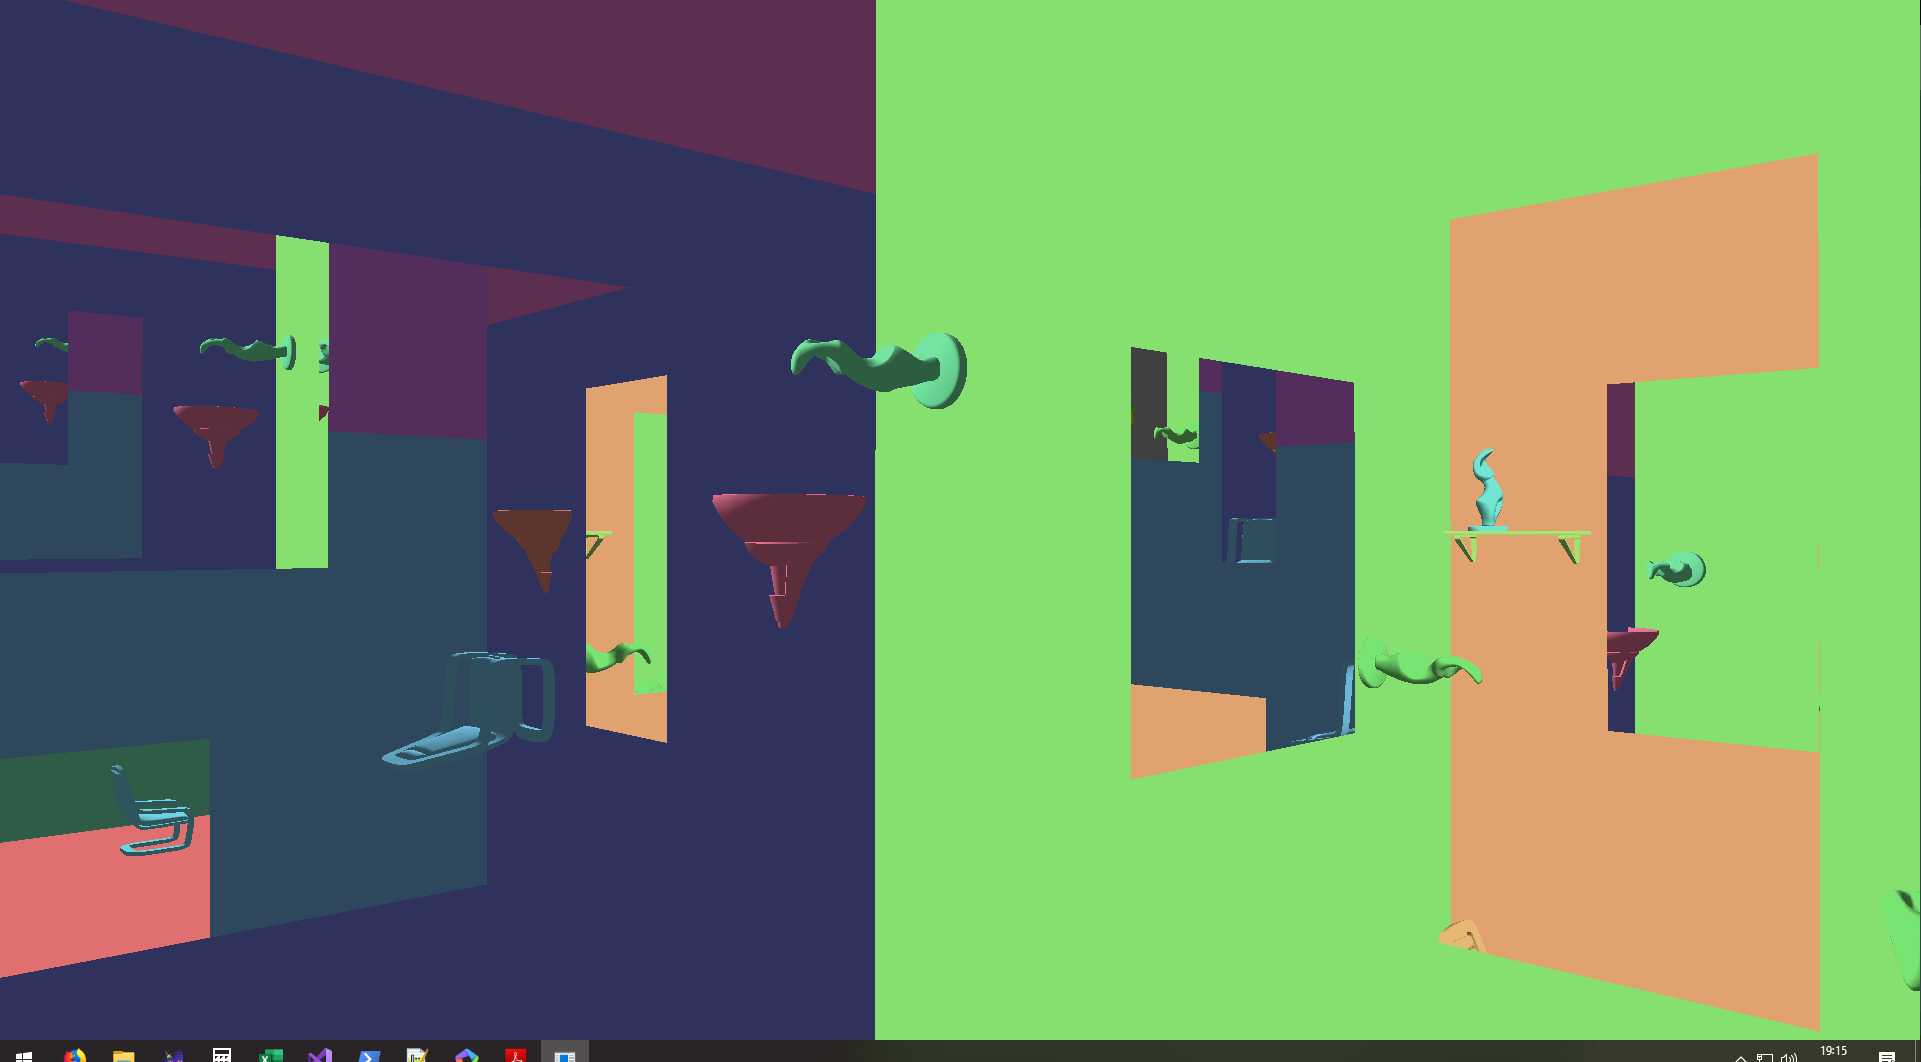
\includegraphics[width=\linewidth]{images/testsnapshot.png}
	\caption{View point for measuring. Maximum visible portal and recusion count to produce the image was 8-6-4-2.}
	\label{fig:perfviewpoint}
\end{figure}

Figure \ref{fig:perfviewpoint} shows the view point of the following measurement. There are two visible portals and a high amount of recursion. While scenes with many more visible portals could be constructed, this serves as a reasonable case. Note that the displayed image does not look the same for all measurements. E.g. some test cases will only show one recursion.

\begin{table}[H]
	\centering
	\begin{tabular}{|l|l|l|l|l|l|}
		\hline
		Test Case   & Average & Median & Min    & Max    & Relative Median \\ \hline
	   %No Recursion& 1.17    & 1.16   & 1.15   & 1.33   & 0.17		   	   \\ \hline
		8           & 2.95    & 2.90   & 2.24   & 3.48   & 1.37            \\ \hline
		8-6         & 8.29    & 8.28   & 7.36   & 8.96   & 6.19            \\ \hline
		8-6-4       & 14.85   & 14.84  & 13.96  & 15.99  & 8.03            \\ \hline
		8-6-4-2     & 24.97   & 24.91  & 23.09  & 27.05  & 8.43            \\ \hline
		12          & 3.02    & 2.98   & 2.36   & 3.51   & 1.39            \\ \hline
		12-12       & 10.76   & 10.75  & 9.99   & 11.56  & 6.30            \\ \hline
		12-12-12    & 55.21   & 55.20  & 54.32  & 56.25  & 7.62            \\ \hline
		12-12-12-12 & 568.21  & 568.20 & 566.05 & 569.51 & 8.63            \\ \hline
		4           & 2.84    & 2.79   & 2.06   & 3.41   & 1.26            \\ \hline
		4-4         & 6.08    & 6.07   & 5.17   & 6.79   & 3.98            \\ \hline
		4-4-4       & 9.45    & 9.45   & 8.08   & 10.48  & 6.69            \\ \hline
		4-4-4-4     & 16.97   & 16.99  & 15.04  & 19.33  & 7.84            \\ \hline
	\end{tabular}
	\caption{Time in milliseconds to render a scene with 12 portals from Figure \ref{fig:perfviewpoint}'s viewpoint, as well as the relative median time compared to rendertimes without objects on the screen.}
	\label{tab:perfviewpoint}
\end{table}

Table \ref{tab:perfviewpoint} shows the rendertimes in milliseconds for the image shown in figure \ref{fig:perfviewpoint}. The last column is the difference to the rendertimes for without objects on the screen from table \ref{tab:rendernothing}. The median is significantly higher, compared to table \ref{tab:rendernothing}. This is especially true for the low recursion measurement. Their median render time increase makes up a significant fractions of their total median render time. This makes sense, as the most objects are only rendered for the first recursion. For later recursions, it is less likely that an object needs to be drawn. This indicates that producing degenerate triangles for objects that do not need to be rendered (see section \ref{section:viewmatrixselection}), actually helps to improve performance. However, this also shows that the base render times from table \ref{tab:rendernothing} are not really reliable. The actual rendertimes depend heavily on the rendered scene. This table alone shows render times up to 4 times more than the baseline (Test Case 8-6). Care needs to be taken when building scenes. The numbers also suggest that the \gls{recursioncount} should likely be limited to 3 instead of the previous stated 4.


\section{Properties of Watertight Portals}
\label{section:watertight}
Special properties of of watertight portals were found during the testing of the implementation. Watertight portals are portals that use an watertight mesh. A watertight mesh, does not have any holes. When looking at a watertight portal, objects behind it will be visible a though it did not exist. Watertight portals, seem as though their did not exists. However, their contents are swapped.

\begin{figure}[h]
	\centering
	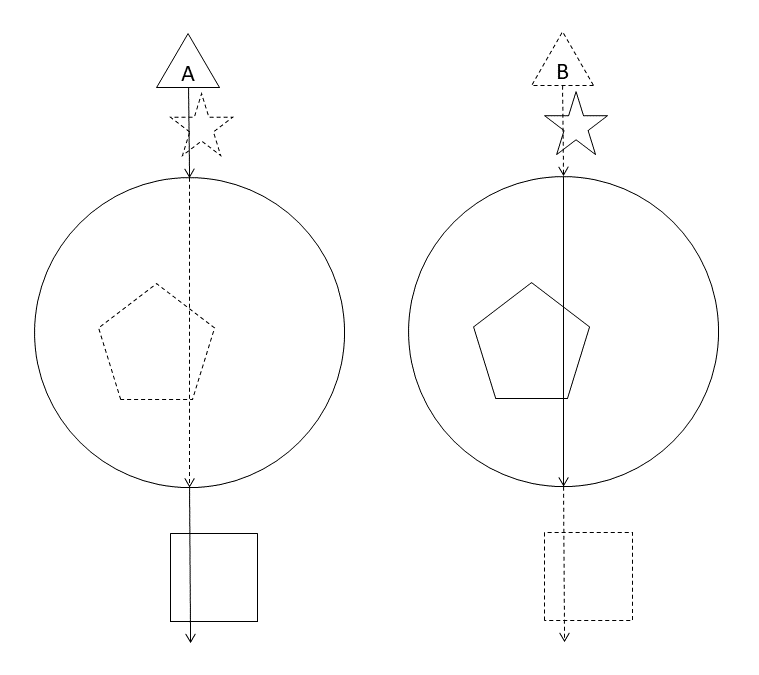
\includegraphics[width=0.8\linewidth]{images/watertight.png}
	\caption{A Watertight Portal Pair}
	\label{fig:watertightportals}
\end{figure}

Figure \ref{fig:watertightportals} show an example of a watertight portal pair. The two big speres are the two endpoints of a watertight portal pair. There are two viewpoints A and B.
There are two approaches to interpret the figure, which both are valid.
The first is that A's view is indicated by full stroked arrows, while B's view is indicated by doted arrows.  Only objects with full strokes can be seen. This is how viewing behaves. The view teleports when passing through the portal, and teleports back when passing it again.
The other is that A and B's view is a straight line. When the view is fully stroked only fully stroked objects are scene and when dotted only dotted objects are seen. This is how it actually looks for A and B.
In this example A can only see the pentagon and the square, while B can only see the star. Only the fully stroked objects are the actual placements of the object. Notice that it looks, as if the are inside both places is swapped.

Static watertight portals, do not really have a purpose. They can't be detected and only the contents are swapped. They might as well not exists and the scene could be built accordingly for the same effect.

When using Watertight portals, they need to be created or transformed during runtime, otherwise they just cost performance without any gain. After discovering this fact, the watertight portals were removed from the implementation's scenes.

However, this property of watertight portals could be exploited. If watertight portals are treated specially, there might be some opportunities for optimization.

\subsection{Holes}
Cutting holes inside an otherwise watertight portal has some interesting properties. As previously mentioned a watertight portal is not really detectable and only serves for switching spaces. However when a hole is cut, the hole would appear as a portal. The hole could be seen as an additional portal, which cancels out the watertight portal. But the watertight portal would not really be visible to the user, so they see only that additional portal, which does not actually exist. This property can be seen in the half sphere portals in the implementation as shown in \ref{fig:nonplanar} in section \ref{section:nonplanar}. The black area in the top image indicates the circular planar hole, which is the only part in the bottom picture which actually looks like a portal. The actual part of the half sphere portal only serves as a border for the swapped space.
\chapter{Performance Improvement Opportunities}
\label{section:performanceimprovements}

Section \ref{section:performancemeasurement} measure the performance of the prototype and discovered some bottlenecks. This section will focus on how the performance could be further improved using this information. Then two additional potential performance improvements are discussed, which are not based on measurements. However

\section{Preventing false Visible Portals}
\label{section:falsevisible}
The manual stencil test introduced in section \ref{section:dynamicportalinstancerendering}, enabled testing portals early, for recursion 0. Portals that fail the stencil test, no longer count as visible portals for the algorithm described in section \ref{section:visibleportalcount}. However, subsequent recursion cannot use early tests, due to the manual stencil and near depth test, which discards fragments. Portals that are occluded by objects still count as visible. Additionally, even with an early test, portals that would be occluded later by other portals still count as visible.

Table \ref{tab:perfviewpoint} from section \ref{section:renderperformance} has shown that there is quite a difference, between rendering nothing and rendering multiple portal recursions. The less visible portals there are, the better the performance.


One way to prevent false visible portals is by running a depth pre pass for the portals. This pass renders all portals, but does nothing but to write depth values. It still performs the manual tests, for stencil and near buffer. Then the portals are drawn again, with an early depth test. For this pass writes to the depth buffer can be disabled. Thus the nearest depth values are already known and only portals that will not be occluded qualify as visible for the visible portal count algorithm.

There is also another possibility, which only needs an additional depth texture, but no pre pass. While  rendering objects a far depth buffer is used, just as always. However, during the portal rendering, this depth buffer is given as input for the portal shaders. They perform an additional manual test for the far depth. Portals still use a regular depth buffer also, so that portals occlude each other correctly. Although portals occluded by other portals still count as visible, portals occluded by objects do not. As the later case is far more likely, this could cut down the amount of false visible portals drastically.




\section{Camera Matrix Improvement opportunities}
The generation of the view matrices, described in section \ref{section:generatingviewmatrices} could be improved. Three areas were found, where the algorithm could be improved.

\subsection{Using view matrices directly instead of camera matrices 0.5}
Currently when calculating the view matrices, first all camera matrices are calculated, after which each of them is inverted to find the view matrices. $C_n$ is the nth camera matrix, $T_n$ is the nth teleport matrix and $V_n$ is the nth view matrix. $C_0$ is the initial camera matrix. This can be written as:

$$C_n = T_{n} * C_{n-1}$$
$$V_n = (C_{n})^{-1}$$

Section \ref{section:perfmatrixcalc} has shown that taking the inverse of the matrices accounts for approximately 2/3 of the total calculation time. The new approach would not need to take the inverse of a matrix. Instead the view matrices can be used directly.
Combining the previous two equation yields:

$$V_n = (T_n * C_n)^{-1} = C_n^{-1} * T_n^{-1}$$

The inverse camera matrices can be substituted by their respective view matrices yielding.
$$V_n = V_{n-1} * T_n^{-1}$$

Results from previous calculation can be reused, the same way as previously. As the inverse of \gls{endpoint} A's teleportation matrix is equal to \gls{endpoint} B's teleportation matrix, no matrix but the initial camera matrix needs to be inverted. If time had permitted it, this optimization would definitely be included in the implementation.

\subsection{Excluding the initial view matrix}
\label{section:noveiw}
Let $Vwv0_n$ be the view matrix for portal n, which misses the multiplication with the initial view matrix. Formally:

$$V_n = V_0 * Vwv0_n$$

$Vwv0_n$ can be defined recursively as:

$$Vwv0_n = Vwv0_{n-1} * T_n^{-1}$$

The advantage of leaving out $V_0$ from the multiplication is that, if all $T$ are constant all $VWV0$ will be constant as well. These matrices only need to be calculated once, instead of every frame. The final calculation to get the real view matrix can be done in the shader. This does not need to be a matrix matrix multiplication, as it the view matrix is used only once in the shader for calculation a vertex's position. The array of these matrices could reside in \gls{gpu} local memory, as they do not need to be changed. Even for scenes with moving portals, this could be a useful optimization, as only the parts that depend on the moved portal need to be recalculated. However, if this really improves performance for a specific implementation needs to be tested.

\subsection{Calculating on the GPU}
Instead of calculating the view matrices on the \gls{cpu}, they could also be calculated on the \gls{gpu}.
This saves the \gls{gpu} bandwidth, as only teleport matrices and the view need to be transferred, instead of an array of every possible combination of portals. Additionally, the indirection described in section \ref{section:viewmatrixselection} can be removed. After the previous visible portal calculation the view matrix can be calculated and written to the correct location. Lastly, access is faster as the matrices are in \gls{gpu} local memory.

The total number of calculated matrices might be more or less on the the \gls{gpu} compared to calculating it on the \gls{cpu}. This  depending on the number of portals on the scene and the number recursion and visible portal counts. 

For example for a scene containing 12 portals 22,620 matrices are needed. This is the amount of matrix multiplications that would be done on the \gls{cpu}. When rendering with visible portal counts of 8-6-4-2, only 632 matrices are actually used at most. Most likely the number will be significantly lower. When only 4 of 8 portals are visible in recursion 0 at most half the previous state amount of matrices will be needed. When combined with the optimizations described in section \ref{section:falsevisible} there will be even less matrices needed. However, the \gls{gpu} would need to calculate the matrix for each fragment of a portal. But the \gls{gpu} does this in parallel so this might not as dramatic. 

This approach increases the \gls{gpu} workload, while reducing \gls{cpu} load. Depending on the current bottleneck, this can be an advantage or a downside. The workload of the \gls{cpu} increase with number of portals in a scene, while the \gls{gpu} workload increases with resolution and the maximum visible portal counts. If the visible portal counts stay the same, at a certain amount of portals in a scene there will be a tipping point.

Lastly this approach can not be used together with the one described in the previous section. Which one to use depends on the nature of the scene. If the portal matrices stay (mostly) the same and there is enough buffer storage available, the previous approach is probably better suited. But for scenes with many moving portals, the matrices must be recalculated anyway, so this approach might be a better fit. 








\section{Dynamic Visible Portals count}
The visible portal count may not only be different for every recursion, it could even change during run time. The only change in the implementation would be to reserve enough space for the indices array and helper array, described in section \ref{section:indexarrayproperties} and \ref{section:helperarrayproperties} respectively. Everting else uses values that can change during run time.

For example dynamically decreasing the visible portal count for recursion 0, while increasing it for recursion 1. This is useful for situations where only one portal is visible, because the camera is directly in front of it.

This this allows for more visible portals during recursion 1. The amount of stencil values used as well as the amount of times the scene is rendered stays roughly the same.

Another application would be dynamically lowering the visible portal counts, if the last frame took to long to render.

\section{CPU Portal Culling}
\label{section:cullingportals}
Table \ref{tab:rendernothing} showed that a high maximum visible portal count can increase the time to render, even if nothing is rendered. Keeping this value low could improve performance drastically. A similar approach to the one suggested by \cite{luebke:1995:portals} could be used.

Each Portal's vertices are multiplied with the view matrix. Next the bounding box is projected into screen space, but the Z coordinate should be left intact, as it is useful for further calculations. Conceptionally the vertices are multiplied with the perspective matrix and then divided by their w component. Then the w gets discarded and the z coordinate is overridden with its original value.

Around the projected points a \gls{aabb} is created, which will be called \gls{psb}. This \gls{psb} is then intersected with the \gls{psb} of the portal it can be seen through. For example, if portal B can be seen through portal A, portal B's \gls{psb} is Portal B's \gls{aabb} intersected with portal A's \gls{psb}.

This intersection is then the portal's actual \gls{psb}. Recursion zero has no parent portal and uses a \gls{psb} from (-1,-1,0) to (1, 1, Infinity) instead for the intersection. If the resulting \gls{psb}['s] volume is zero, the portal is not visible and can be discarded. Otherwise, its \gls{psb}['s] max z value is set to positive infinity as the last step.

%Watertight portals can also be handled in a special way by keeping their max z value. Then when its other endpoint inside them is processed instead of calculating the other endpoint's \gls{psb} it is given its parent's \gls{psb}, but with an infinite max z value. 

%This works, because for portals to be visible they must be inside the watertight portal. Otherwise,


With this the visible portal count for a recursion could be conservatively estimated. This will usually be a much lower number than the fixed one. Furthermore the visible portal count does not need to be fixed for a whole recursion. Each rendered \gls{portalset} could use a different max visible portal count, instead of all using the highest count. This could improve performance even further.

One thing that must be noted is that the way view indices and stencil values are calculated must fundamentally change when implementing this approach. This might also mean passing additional push constants.

Culling portals does not make the dynamic calculation of actual visible portals obsolete. Portals may still be occluded by scene objects. Producing degenerate triangles for objects drawn inside occluded portals, can still improve performance as table \ref{tab:perfviewpoint} has shown.

\section{Portal Frustum Primitive Clipping}
\label{section:portalprimitiveclipping}

When drawing recursion 1 and onward only a small part of the scene will be drawn. Although the near buffer allows for correct drawing, unneeded fragments are still generated. One good way of reducing the produced fragments is by allowing fewer triangles to be passed to the rasterizer. 

One way to achieve this is by decreasing the clip volume. Regularly the view frustum is used as clip volume for primitive clipping. However, as the portals is only at part of the screen primitives should be clipped to this much smaller volume. This volume is referred to as \gls{portalfrustrum}. The \glspl{psb} introduced in section \ref{section:cullingportals} can be used to calculated the frustum. The \gls{psb} must be available in the vertex shader. The individual clip distances are calculated via subtractions in the vertex shader. Note that while Z can be directly used, the  x and y coordinate must be in the same space as the ones of \gls{psb}. Either the \gls{psb} is transformed into view space, using the the vertex's z. Or the vertex's x and y coordinates are projected into screen space. The only difference between those two possibilities is that the clip distances are scaled by z. This should not matter for the primitive clipping \cite{khronos:vulkan:spec1.1}.  Which variant is faster would need to be investigated. The regular clip planes for the regular view frustum can then also be disabled, as the \gls{portalfrustrum} is a subspace of it.

\section{CPU Portal Frustum Culling}
\label{section:portalfrustumculling}
The results from section \ref{section:cullingportals} can be reused to perform a variant of frustum culling. There are multiple ways to do this. One would be to unproject and transform the \gls{psb} to create worlds space portal frusta. Then commonly used frustum culling can be performed.

Frustum culling can also happen in view space  with its own advantages and disadvantages. The actual test is simpler, as \glspl{aabb} can be used. However, the the bounding box must first be transformed into the perspective coordinate system \cite{assarsson:2000:optimized}.


This test can be done against the \glspl{psb} directly. To reduce the amount of points that need to be transformed, a bounding sphere is used. However this works only if all scaling is uniform. The center of the bounding sphere is first transformed into camera space. Then a minimal \gls{aabb} can be build around the sphere. Initially only the \gls{aabb}['s] z axis is tested against the \gls{psb}. This is valid, as the z axis of the \gls{psb} is in camera space. If this test fails the object can be culled and not further test is needed. Otherwise the x and y need to be tested. To test x and y  the coordinate systems for \gls{aabb} and \gls{psb} must match, similar to described in section \ref{section:portalprimitiveclipping}. Which approach is better needs to be investigated. This sections will describe transforming \gls{psb} into camera space. 

\begin{figure}[h]
	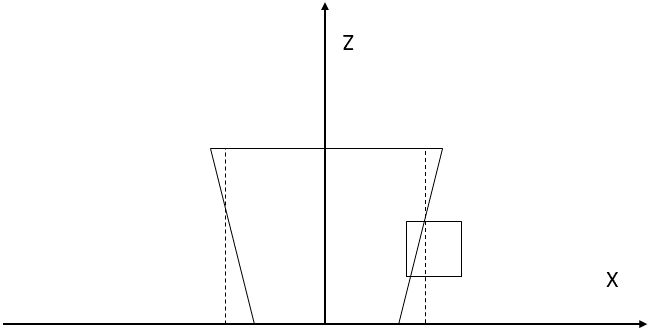
\includegraphics[width=\linewidth]{images/frustumbox.png}
	\caption{Top view of the culling processes. The trapeze represents the portal frustum. The square represent the bounding box of the object. The dotted rectangle can be used instead of the portal frustum for the culling. }
	\label{fig:frustumbox}
\end{figure}

Figure \ref{fig:frustumbox} shows the portal frustum in camera space as well as the \gls{aabb} of the object. Instead of testing against the frustum, the test is performed against the dotted rectangle, which is also an \gls{aabb}. It is constructed by unprojecting the \gls{psb}['s] x and y with the object's \gls{aabb}'s far z, as this is the point where the frustum is the biggest, while still being in the object's \gls{aabb}'s z range. Only x and y need to be tested against this box, as z was already done.


The instance count of the object when rendered should correspond to the amount of times the  test succeeded. However, the gl\_InstanceIndex cannot be used directly anymore to find the correct view matrix and stencil value. Additional information must be passed to the vertex shader. For example an array of stencil values/view matrix accessed via gl\_InstanceIndex.

\section{Draw Indirect}
Instead of using \textit{drawIndexed} an implementation could use \textit{drawIndexedIndirect}. This allows only using a single draw call to render all objects multiple times. Additionally, portal fragment shaders could manipulate the values in the draw indirect buffer. If less portals than the maximum visible \gls{portalcount} is visible, there can be fewer instances. Similar to the approach of section \ref{section:cullingportals} the downside is that \textit{gl\_InstanceIndex} cannot be used directly anymore in the shaders, and the real value must be obtained via buffer writes and reads. But when implemented correctly this no unneeded instances are drawn. The current implementation produces degenerate triangle instead of skipping the whole instance. It needs to be measured if this approach actually improves performance enough compared to the current implementation, to be worth the extra work. Additionally, adjusting instance counts could be difficult or not yield much benefit when this approach is combined with the approaches of section \ref{section:cullingportals} and section \ref{section:portalfrustumculling}.

\section{Reduce depth attachment count}

In section \ref{section:dynamicportalinstancerendering} a manual stencil buffer was introduced. This means the depthstencil attachment is now exclusively use for the far depth buffer. When rendering portals the depth values are written into the write near buffer as well as the far depth buffer for the depth test. After this the rendering of all \gls{portalset} the depth buffer's contents are no longer needed and must be cleared. The values in the far depth buffer and the write z buffer are nearly the same. The only difference is that the far depth buffer contains the depth values, from rendering the objects. However, for later sub passes there is no real difference, as the manual stencil test discards fragments that would read at locations, where not portal was drawn. This means that the far depth buffer can be used instead and no write near buffer is required. One less texture is needed. However, other means must then be found to detect portal front and back faces, as described in section \ref{section:portalzfighting}.

\chapter{Visual Improvement Opportunities}
Performance is not the only area where the prototype can be improved. Currently the prototype lacks support for lights and transparent objects. This section will cover how these could be implemented and what difficulties arise in the presence of transformative portals.

\section{Shadows and Lighting}
Due to time reasons the prototype has no shadows and only one directional light was implemented. This section covers a approach that would have been used, if time had allowed. For a portal to appear seamless care must be taken when lighting. Otherwise for instance shadows could appear cut of or appear out of nowhere in the presence of a portal.

\subsection{Portal Shadow Mapping}
One approach would be a modified version of shadow mapping. In the presence of transformative portals a occluder is not enough for an object to be considered in the shadow. Light might travel through a portal and light it indirectly. When rendering shadow maps the same approach can be taken that is used to render the scene with portals, i.e. multiple recursions, but from the lights view. However in addition to the depth values, the view matrix used for rendering a fragment must be saved as well. This can should be in form of an index to save space, but it must be possible to retrieve later. 

Then when rendering the actual scene, the shadow test is performed. However, as it is not known whether the light travelled through a portal the position on the shadow map can not be calculated directly. It is possible that the same fragment can be lit by the same light multiple times, using different portals. They need to be regarded as separate dynamic lights which share their shadow map.

For each portal combination the light could have travelled through, the corresponding teleport matrices must be applied to the light position. Then the position on the shadow map is calculated using that transformed light position. The shadow map's matrix is compared against the matrix used to transform the light position. If they do not match this is treated the same as if the depth does not match. Then the regular depth check is performed.

\subsection{Lighting}
For lighting only a directional light was implemented. With directional light it is the least noticeable when it is not handled correctly. Especially when portals are placed that the direction light is almost parallel to them.
Lighting is also difficult its possible that a fragment can be lit by the same light multiple times. For shadow casting lights, information from the shadow map can be used to detect from where a fragment is lit. If for a specific light portal combination the object does not lie in the shadow, the lights position used for accessing the shadow map can be used for lighting calculations.

However for lights without shadow maps light seems impossible. Lighting a fragment for possible portals the light could have travelled through would create wrong results and is computationally expensive. 


\subsection{Portals as Light Source}
\label{section:portalsaslights}
Performing doing correct lighting and shadows is expensive. Depending on the use case a potential solution would be to perform lighting and shadowing as though portals did not exist. To hide the seams at portal locations, the portals could behave as a very bright point light. Fragments would appear almost fully lit and shadows would fade out near portals. All fragments close to the portals would be lit the same and not seams would be visible.

However, this has the downside that the location of portals is very visible. If this is not desired the scene must be designed in a way that there are always lights near portals or only use one directional light without shadows and no other light sources.


\section{Transparent Objects}
Transparent object are not supported in the implementation, but there is nothing that would stop implementing them. They would be rendered very similar to regular approaches. First everything opaque is rendered, including all portal recursions. After everything is drawn the transperent objects are drawn back to front, starting from the last recursion and ending with the initial recursion \cite{lecture:portalProblems}.

However, the far depth information of all recursions must be saved. Otherwise, the whole scene must be redrawn to get the depth information. This could be done by saving using different depth buffers and not clearing them. Or By using a depth prepass for portals and when rendering the again setting the depth value to infinite far away, instead of clearing the whole buffer. The near buffer can be recreated by drawing the portals again as drawing a few portals is likely far less expensive compared to drawing the whole scene and might not be a huge concern. Alternatively, the far buffers for each recursion could just be saved, but this requires more textures.


\chapter{Portal Capability Improvement Opportunities}
The last area of improvement is the capability of portals. While the portal in the prototype are already functional, they are lacking in a few areas. Improving the capabilities of portals broadens the spectrum of portal applications. 


\section{Portal Physics}
\label{section:portalphysics}
The implementation currently only supports collision for the camera. Depending on the use case for portals, portal physics are need. There are several problems that must be solved to allow for realistic portal physics.

\subsection{Portal Edges}
Portals that are not completely place on solid objects either must have collision on their edges or allow slicing objects into pieces.

\begin{figure}[h]
	\centering
	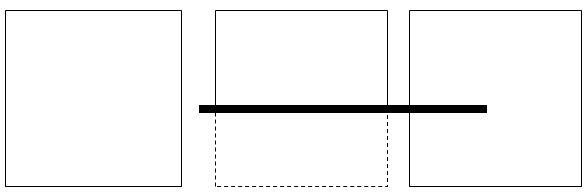
\includegraphics[width=\linewidth]{images/edgecollision.png}
	\caption{A box represent an object, while the thick line represents a planar portal. It is not clear what should happen to the right object}
	\label{fig:edgecollision}
\end{figure}

Figure~\ref{fig:edgecollision} illustrates the problem that can occur. The left box passes the portal, the middle box goes through the portal, with the dotted  part being present at another location. However, It is not clear what should happen to the right box. The right box case could be  be prevented via collision on the portal edge. Or the box could be sliced by the portal edge so that one part goes through the portal, while the other passes it. Watertight portals do not have edges, so this problem cannot occur for them.

\subsection{Halfway through Objects}
As objects are not point it is possible that only part of an object has passed the portal. The two parts of the object must be exists two different locations. Just duplicating the object is not enough however. It must also be insured that an object piercing a portal from the front, cannot be seen or interacted with from the back. Additionally the physics state must the same for both parts. Furthermore similar care must be taken for the player's avatar. If the player is halfway through the portal, they should not see part of their avatar directly at their viewing location. Some of this problems can be seen in the presentation of \textcite{lecture:portalProblems}.


\section{Non-Translating Portals}
The implemented portals have two endpoints. Objects Touch on endpoint, get move to the other. However, it is also possible that the portals don't move the object. In this case there are no two end points. It is just one portal.

Entering the portal would apply a operation (e.g. multiplying by matrix), leaving it applies the inverse operation. Instead of rendering two endpoints, only one portal is rendered. Back and Front face detection needs to be used to decide which operation to apply.

This works mostly only for operations which don not move the position of an object. One exception would be a rotation, but portal shape looks the same after applying the rotation to it. E.g. a sphere could allow for any rotation. A cube only for rotation in intervals of 90 degrees. Inverting or the scale of an object would another case.



\subsection{Arbitrary Operations}

In the implementation the portals only apply transformative operations in using matrices. Non-Translating Portals would allow for portals that can apply such operations, without needing to also translate an object.

A portals operation could change render parameters. These parameters are store similar to the view matrices. One example inspired by \cite{borst:2009:real} would be marking pixels if one parameter currently has a specific value. Later in a post process the marked pixels could be modified. Another example inspired by magic lenses, would be a parameter which decides which objects to render. Some objects will only be visible, while the parameter has a specific value.

Inspired by the works of \textcite{ryall:2005:temporal} and \textcite{tiesel:2009:composable}, another very interesting form of a non translating portal would be a temporal portal. Instead of moving through space it moves through time. In a temporal portal the past could be seen and by travelling through it objects could time travel. However, even more care than described in section \ref{section:portalphysics} must be take, such as objects colliding with its past self, changing the presence by changing the past etc.






%\section{Form changing portals ?}
%{multiple portals, represented by one mesh}
%{portals as mathematical function, implicit surfaces }

%\section{Change portal connections ?}



\section{World Wrapping}
World wrapping enables infinite world, by repeating itself. When something moves outside one end of the wrapped world it is teleported to the opposite end. It is possible to implement world wrapping using the current implementation's transformative portals. However, portals used for world wrapping can be seen as very specific kind of portal. This allows for special optimizations: Such portals are defined as an pairs infinite planes. The World exists only inside those planes. No object is outside the subspace defined by the plane pairs. 

The stencil test is not needed, as the only the repeated scene will be drawn at that location. The near buffer is also not needed, as the multiple scenes can not overlap each other. This means drawing the actual portals is not necessary. All world instance can be drawn at once, using instanced drawing, with each world instance using the corresponding view matrix.

However, if portals are already present its probably better to just define big portal planes. Otherwise, the process that was just described needs to be used also for each world that is drawn for a portal.


\chapter{Conclusion}

%\section{Implementation summary}

Previous works used a depth first approach to render transformative portals. This thesis present another approach by using breadth first. Additionally it supports arbitrary portals defined by triangle meshes. While arbitrary portals are becoming more common, they are not supported everywhere.

On the authors machine, the implementation performed quite well. Scenes with 10 or more portals ran smoothly. However, in most settings the \gls{recursioncount} cannot be higher then four. Higher recursion counts took increasingly much longer to render exceeding the maximum time available for real time applications.



The implementation used many techniques found in previous works to render transformative portals. However, two key improvements could be implemented which the author has not yet seen in other works.

The first is the visible portal count algorithm. It allows to perform occlusion query-esque operation during the execution of a fragment shader. This allowed to many more portals in a scene, as long as only a limited number of them were visible. While this could be used in depth first portal rendering, the author has not yet seen something similar implemented.

The second is the use of instanced drawing. While instanced drawing is commonly seen, the author has yet seen its use in the context of transformative portals. Instanced drawing helped to improve performance by drastically reducing the amount of operations sent to the \gls{gpu} improving the overall performance significantly. Upon the introduction of instanced drawing, the time to render was only a sixth of the time before. Instanced drawing is probably one of the biggest benefits of breadth first portal rendering.

Furthermore, the implementation was created using only a single renderpass, with multiple subpasses. This potentially allows the \gls{gpu} to optimize. The number of subpasses needed scales linearly to the \gls{recursioncount}. However, this thesis only proved that breadth first is a viable approach, which allows for special improvement opportunities. It does not indicated whether depth or breadth first performs better in different situations.

One downside of the breadth first approach was, that drawing instanced prohibited the use of the regular stencil test. As the reference value cannot be changed between instances, the implementation resorted to manually stencil testing and discarding fragments in the shader. This prohibited using early fragment tests. This was not seen as much of a downside, as the dual depth buffer also required also required manual testing and discarding, prohibiting early fragment tests anyway. However, for applications that do not need to use a dual depth buffer, this can be considered a downside. Furthermore, the use of manual test requires inserting them in every shader, which is inconvenient.

Another downside is that due to the way the view matrices are calculated, the implementation still has a limit of maximum portals in a scene. They still affect performance, even if they are not visible. However, this problem should be relatively easy to fix in future. Many optimisations discussed in section \ref{section:performanceimprovements} would either speed up the calculation or reduce the needed matrix count considerably.

A interesting discovery were portals defined by watertight meshes. They are not very useful as static portals, but when modified dynamically allow for effects such as swapping or rotating subspaces. Additionally, the holes of almost watertight portals behave as a portal for the user, while the actually portal seems not to be present. But in reality the reverse is true.


\section{Possible Improvements}

While the current version of the prototype has already has some use cases, it there are still many improvement opportunities. However, not every improvement opportunity is useful for every application. Three directions were identified.

In the visual area the prototype can be improved by supporting more than a single directional light for shading and adding shadows. Depending on the application these may be implemented in a less exact way to improve performance. The resulting artefacts can be hidden with well placed light sources. Additionally support for transparent objects can be added.

The portal's capabilities can be improved. Non-translating portals, portals with more than just transform changes and physical portals are important aspects not present in the implementation. This increases the potential for using portals in games or similar applications. Very unique game concepts would be possible, which can set such games apart from competition.

Lastly the performance of the implementation can be improved. Not all performance opportunities are equal. The most performance is likely to be gained by adding culling techniques. Performing visibility culling on portals (see section \ref{section:cullingportals}) seems to be the most important one. Additionally, the results can be reused for the other culling techniques. Furthermore, it the approximate count of drawn portals is known on the \gls{cpu}. This decreases the need for other performance opportunities, such as calculating view matrices on the \gls{gpu}. Another important opportunity is to improve the calculation of the view matrices by removing the need for matrix inversion. This seems to provide some gain for almost no work and is strongly recommended.

The introduction of visibility culling might have strong impact on the prototype and some of the choices need to be revisited. Unless extra steps are taken to prevent false visible portals (see section \ref{section:falsevisible}) the dynamic calculation of visible portals might be almost obsolete. In such a case the extra work introduced via indirections and synchronisation might not be worthwhile.

Additionally there are some possibilities that would require changes in the graphics \gls{api}.

At the moment it is not possible to allow early fragment testing, as manual checks against the near buffer need to be performed in the shader. However, if in the future the depth test allows the use of a near buffer some decisions there are some improvement opportunities. It might be worthwhile to remove instanced drawing, in favour of early fragment tests. If stencil export for shaders prior to rasterisation are available, instancing could still be used.

Another opportunity would be the separation of the comparison and write operations of a depth test and stencil test. If the writes only happen after a fragment shader is executed without calling discard, the comparison operation could happen early.

\section{Possible Applications}
The work of this thesis can probably best applied to video games. Portals can not only only serve a gameplay mechanic, but be used for other purposes as well, such as seamless transitions between scenes similar to the work of \textcite{schmalstieg:1999:sewing}. Video games have only used a sparingly amount of portals. The breadth first approach might offer better performance, allowing for a higher portal count. However, as previously stated this would need to be tested first.

Mirrors are a form of a portal that are much more common than transformative portals. The techniques described in this thesis can be applied to them as well. In addition, mirrors are often plane shaped. The the near buffer could be replaced by user defined clip planes.


\subsection{Improving Portal based occlusion culling}
The technique use to calculate previous visible portals could be adapted and used together with portal based occlusion culling. Objects within cells are rendered using draw indirect. This allows changing the instance count of the objects and can effectively disable them. All objects within are cell are only enabled, if at least a fragment of the corresponding portal is drawn. This can be achieved by initially setting the instance count to 0 for all object. Then in a portals fragment shader the instance count can be set to 1, which only happens if at least one fragment is drawn.

Depending on  available \gls{gpu} extension this approach can be further improved. When using Vulkan the extension VK\_EXT\_conditional\_rendering can be used. This removes the need for an draw indirect buffer and looping over all its elements and setting the instance count individually \cite{khronos:vulkan:spec1.1}.

Another useful extension for this purpose are representative fragment tests. If any primitive produces one or more fragments that all pass the fragment test one or more of those fragments are chosen. All other fragments are discarded. As its only important to detect whether or not at least one fragment is visible, this can reduce the amount of unneccesary fragments. The test can be enabled with GL\_NV\_representative\_fragment\_test and VK\_NV\_representative\_fragment\_test for OpenGL \cite{khronos:openGL:representative} and Vulkan\cite{khronos:vulkan:spec1.1} respectively.


%\section*{Image based portal rendering - likely does not work well}
%For each portal render its view into texture, if the view contains another portal, save the id and uv coordinates. Make a copy of the textures. Then process textures again, overwriting previously marked portals. This is done by fetching the pixel with the saved uv coords from that texture. This pixel may be a colour or could be a portal mark. Repeat this process until there are no more portal markings or when threshold is exceeded.
%Bad scaling with maxiumum portal count
%Good scaling with recursions: as drawing a portals contents also draws its recursion contents, doubling the amount of recursions with each step -> 1,2,4,8,16...
%Might look ugly, wrong perspective


%For debugging OpenGL offers debug output to obtain details about errors, performance warnings and other useful information. They can be obtained via a debug message callback or by querying them from a message log \cite{khronos:openGL:spec4.6}. In Vulkan validations layers are used for finding errors. In Vulkan \gls{api} calls can be intercepted by layers. They perform whatever operation defined by their implementation before maybe passing them to the actual function. Validation layers are layers w

%They validate the parameters, before passing them to the actual function. How errors are reported depends on the implementation of the layer.. Multiple layers can be active and are called each one sequentially before calling the actual function. \cite{khronos:vulkan:spec1.1}












